% Detailed technical report (ESC113M extended project, V3). Formatting only: at the
% author's request the layout follows the author's CHE453 (IIT Kanpur) course-report template;
% no CHE453 content is used. Template features reproduced:
% LaTeX article class, 11 pt Computer Modern (OT1), US Letter, 1 in margins,
% running header (title left, page number right) with a 0.4 pt rule, a
% separate vertically centred cover page, a page-1 title block with project
% table, author table (booktabs) and objectives list, numbered sections,
% indented paragraphs, booktabs tables with bold "Table n:" captions above,
% "Figure n:" captions below, numbered equations and a numbered reference list.
% Every number is read from generated/values.tex (written by `python run_all.py`).
\documentclass[11pt,letterpaper]{article}
\usepackage[margin=1in,headheight=14pt]{geometry}
\usepackage{amsmath,amssymb}
\usepackage{booktabs,array}
\usepackage{graphicx}
\usepackage{float}
\usepackage[labelfont=bf,font=small,labelsep=colon]{caption}
\usepackage{enumitem}
\usepackage{fancyhdr}
\usepackage[hidelinks]{hyperref}
% PDF metadata (kept in step with REPORTS in reports/build/build_reports.py)
\hypersetup{pdftitle={Dynamic Modelling, Reliability-Based Optimisation and Adaptive Operation of a Jacketed Stirred-Tank Cooling Process},
  pdfauthor={Nithin D H},
  pdfsubject={Detailed technical report, ESC113M extended project (V3), Department of Chemical Engineering, Indian Institute of Technology Kanpur},
  pdfkeywords={jacketed stirred tank; RK4; Monte Carlo; chance-constrained optimisation; Sobol sensitivity; adaptive operation; simulation study},
  pdfcreator={pdfLaTeX},
  pdfinfo={Institution={Department of Chemical Engineering, Indian Institute of Technology Kanpur}}}
\graphicspath{{figures/}}
\input{generated/values.tex}

\pagestyle{fancy}
\fancyhf{}
\fancyhead[L]{Detailed Technical Report --- Jacketed Stirred-Tank Cooling}
\fancyhead[R]{\thepage}
\renewcommand{\headrulewidth}{0.4pt}
\captionsetup[table]{skip=4pt}
\setlist{itemsep=1pt,topsep=3pt}
\newcommand{\mdot}{\dot m}

\begin{document}

% ---------------------------------------------------------------- cover page
\begin{titlepage}
\vspace*{\fill}
\begin{center}
{\LARGE\bfseries Detailed Technical Report}\\[14pt]
Dynamic Modelling, Reliability-Based Optimisation and\\
Adaptive Operation of a Jacketed Stirred-Tank Cooling Process\\[10pt]
ESC113M Computational Engineering --- Extended Project, Version 3\\[6pt]
Nithin D H, Roll No.\ 230708\\[6pt]
Indian Institute of Technology Kanpur\\[22pt]
Extension of the original ESC113M stirred-tank cooling model.\\
Every number in this report is generated by the accompanying code.
\end{center}
\vspace*{\fill}
\end{titlepage}

% ---------------------------------------------------------------- page-1 title block
\setcounter{page}{1}
\begin{center}
{\LARGE\bfseries Detailed Technical Report}\\[8pt]
Course: ESC113M (extended project)\\[3pt]
Version: 3\\[3pt]
Author: Nithin D H
\end{center}
\vspace{4pt}
\noindent\rule{\textwidth}{0.4pt}
\vspace{2pt}

\noindent\begin{tabular}{@{}p{2.8cm}p{13.4cm}@{}}
\textbf{Project title} & Dynamic Modelling, Reliability-Based Optimisation and Adaptive Operation of a Jacketed Stirred-Tank Cooling Process\\
\end{tabular}

\vspace{6pt}
\noindent\textbf{Author}\\[2pt]
\begin{tabular*}{\textwidth}{@{\extracolsep{\fill}}lll@{}}
\toprule
Name & Roll No. & Base project\\
\midrule
Nithin D H & 230708 & ESC113M stirred-tank cooling model (RK4)\\
\bottomrule
\end{tabular*}

\vspace{6pt}
\noindent\textbf{Objectives for this report}
\begin{enumerate}[leftmargin=*,label=\arabic*.]
\item Extend the single-state cooling model of the original ESC113M project to coupled liquid and jacket-coolant energy balances with a finite, continuously supplied coolant inventory and an operating-condition-dependent heat-transfer coefficient.
\item Solve the model with the classical fourth-order Runge--Kutta (RK4) method and verify it against the exact matrix-exponential solution and an energy balance.
\item Find the agitator speed and coolant flow that cool the liquid to \(T_{target}=355\) K within 1800 s at minimum auxiliary electricity, first deterministically and then with a 95\,\% reliability requirement under parameter uncertainty and a physical pump limit.
\item Assess an adaptive operating policy that estimates the heat-transfer conductance from early temperature data, and test how far the conclusions depend on the assumed model structure.
\end{enumerate}

\section{Executive Summary}

This report extends the original ESC113M project, which cooled a perfectly mixed liquid against a coolant held at 300 K, into a two-state model in which the jacket coolant warms up, the overall heat-transfer coefficient depends on agitator speed and coolant flow, and the agitator and pump consume electricity. The extended model is used to choose an operating point that cools 500 kg of liquid from 370 K to 355 K within 30 minutes. Version 3 corrects five problems found in an independent review and audit of version 2: the simulated coolant flow could exceed the pump limit, the pump energy used the commanded rather than the delivered flow, one design decision was taken after looking at the validation data, one figure annotation mixed two different quantities, and the local sensitivity study perturbed the flow above the pump limit. Every reliability figure in this version comes from a validation set that was generated for the final release and examined only once. All results below come from the corrected model.

\subsection{Key results}
\begin{itemize}[leftmargin=*]
\item \textbf{The coolant side matters.} At the reference point (300 rpm, 0.20 kg/s) the original constant-coolant model predicts \vTOrig\ K and meets the target; the coupled model predicts \vTBase\ K and fails it. The jacket warms to \vPeakTJBase\ K, and the coolant heat-capacity rate acts as a resistance in series with the wall, reducing the effective conductance by \vUAEffDrop\,\%.
\item \textbf{A nominal optimum is only half reliable.} The minimum-energy setting that just meets the target deterministically is \vNomRpm\ rpm at the 0.50 kg/s pump limit (\vNomE\ kWh per batch), but only \vNomPass\,\% of uncertain batches reach 355 K.
\item \textbf{Recommended fixed setting: \vRecRpm\ rpm at a commanded \vRecM\ kg/s.} It was selected on \vNOpt\ optimisation batches with a lower-confidence-bound reliability rule and validated on \vNVal\ independent batches: P(pass) = \vRecPass\,\% (95\,\% CI \vRecLo--\vRecHi\,\%, one-sided lower bound \vRecLB\,\%), expected auxiliary electricity \vRecE\ kWh per batch. Under the corrected model the version-2 recommendation (285 rpm) reaches only \vVTwoRecPass\,\% and no longer meets the requirement.
\item \textbf{Adaptive operation.} Estimating the heat-transfer conductance from ten minutes of noisy temperature data and then setting the agitator speed reaches \vAdPass\,\% reliability (lower bound \vAdLB\,\%) at a mean \vAdMeanE\ kWh per batch, \vAdSave\,\% less than the fixed setting. This is a simulation result; \vAdCap\,\% of batches hit the 600 rpm limit and the gain depends on knowing how the coefficient scales with speed.
\item \textbf{Model structure is the largest remaining uncertainty.} If the coefficient depended more weakly on operating conditions than assumed, the recommended setting would pass only \vWeakFixed\,\% of batches and no fixed setting within the bounds could reach 95\,\%. Calibrating the heat-transfer closure is therefore the first experimental priority.
\end{itemize}

\section{Background and Motivation}

Batch products are frequently cooled in a jacketed vessel to a hold or discharge temperature before the next operation. The temperature affects reaction rates, viscosity and product quality, and the cooling step is usually constrained by a batch time. An operator therefore needs to know which combination of agitation and coolant flow will reach the target in time, how much electricity it costs, and how confident one can be that a given batch will make it.

The original ESC113M project modelled the liquid with a single first-order ordinary differential equation and a coolant fixed at 300 K, solved it with RK4 and compared the result with the analytical solution [11]. That model is exact for its assumptions, but it treats the jacket as an infinite heat sink. A real jacket holds a finite amount of coolant that is replaced at a finite rate, so the coolant warms as it removes heat and the driving force falls. The model also has no operating variables: the heat-transfer coefficient does not respond to agitation or coolant flow, so it cannot be used to choose an operating point.

This project keeps the same tank, liquid charge, heat-transfer area, inlet temperature and 1800 s horizon, and adds what is needed to make the model useful for an operating decision: a dynamic jacket, a closure for the heat-transfer coefficient, an electricity model, and a statistical treatment of uncertain inputs.

\section{Problem Statement and Objectives}

The design question is: \emph{which agitator speed \(N\) and commanded coolant flow \(\mdot_{cmd}\) cool the liquid from 370 K to 355 K or below within 1800 s at the lowest auxiliary electrical energy, and with what probability does a batch succeed when the heat-transfer coefficient, jacket inventory, delivered coolant flow and initial temperature are uncertain?} The 355 K target is an illustrative constraint chosen close to the 30-minute result of the original model; it is not a plant specification. The specific objectives are listed on page~1. The required reliability is 95\,\%, demonstrated on data not used to select the design.

\section{System Description}

The system is a closed, well-stirred batch tank containing 0.50 m\textsuperscript{3} of a water-like liquid. Heat flows through 2.0 m\textsuperscript{2} of wall into a surrounding jacket. Coolant enters the jacket at 300 K and leaves at the jacket temperature. The coolant loop is driven by a pump through a flow-control valve; the pump can deliver at most \(\mdot_{max}=0.50\) kg/s. A turbine impeller of 0.30 m diameter, driven through a variable-speed drive, agitates the liquid at 100--600 rpm. The tank geometry is not specified in the original project; if the liquid height equals the tank diameter, the tank diameter is \vTankD\ m and the impeller-to-tank diameter ratio is \vDT, a common proportion.

\section{Modelling Assumptions}

\begin{enumerate}[leftmargin=*]
\item The liquid is perfectly mixed and described by one temperature \(T_L\). The batch is closed, with no reaction, evaporation or heat loss to the surroundings.
\item The jacket coolant is one well-mixed inventory \(M_J\) at temperature \(T_J\), which is also the outlet temperature. Section~\ref{sec:modelform} shows that this is the conservative limit of jacket mixing.
\item Densities and heat capacities are constant. Over 300--370 K the density of water falls from about 996 to 960 kg/m\textsuperscript{3} and its heat capacity rises from about 4.18 to 4.21 kJ/(kg\,K); the constant values used introduce errors of at most 4\,\% and 1\,\%.
\item The wall heat capacity is neglected and heat transfer is described by one overall coefficient \(U\) on area \(A\).
\item \(U\) follows an assumed power law in agitator speed and coolant flow (Section~\ref{sec:closure}).
\item The commanded coolant flow is delivered by a flow-control loop with a proportional error and a hard upper limit equal to the pump capacity (Section~\ref{sec:actuator}).
\item Agitator and pump electricity follow standard scaling relations with constant, assumed efficiencies. Chiller or cooling-tower electricity, water cost and control power are not included; the energy reported is \emph{auxiliary} electricity only.
\item The uncertain inputs are independent and normally distributed with assumed spreads (Section~\ref{sec:mc}).
\end{enumerate}

\section{Mathematical Formulation}

\subsection{Energy balances}
An energy balance on the liquid gives the rate of change of its sensible enthalpy as the heat flow to the jacket,
\begin{equation}
M_L C_{p,L}\,\frac{dT_L}{dt} = -\,U A\,(T_L - T_J), \label{eq:liquid}
\end{equation}
and a balance on the jacket inventory, with equal inlet and outlet mass flow \(\mdot\), gives
\begin{equation}
M_J C_{p,C}\,\frac{dT_J}{dt} = U A\,(T_L - T_J) + \mdot\, C_{p,C}\,(T_{in} - T_J), \label{eq:jacket}
\end{equation}
with \(T_L(0)=T_0=370\) K and \(T_J(0)=T_{in}=300\) K. The heat-transfer term appears with opposite signs in the two equations, so the heat leaving the liquid enters the jacket. Adding the two equations and integrating from 0 to \(t\) gives
\begin{equation}
M_L C_{p,L}\,[T_0 - T_L(t)] = \int_0^t \mdot\,C_{p,C}\,(T_J - T_{in})\,dt' + M_J C_{p,C}\,[T_J(t) - T_{in}], \label{eq:firstlaw}
\end{equation}
which states that the enthalpy lost by the liquid equals the heat carried out by the coolant plus the heat stored in the jacket. Equation~\ref{eq:firstlaw} is used as a numerical check in Section~\ref{sec:energy}. Since \(T_J < T_L\) at all times, \(T_L\) decreases monotonically, so the requirement ``reach 355 K within 1800 s'' is equivalent to \(T_L(1800\ \mathrm{s}) \le 355\) K.

\subsection{Heat-transfer closure}\label{sec:closure}
To give the model operating variables without adding a hydrodynamic model, the overall coefficient is scaled from its reference value,
\begin{equation}
U = U_{ref}\left(\frac{N}{N_{ref}}\right)^{e_N}\left(\frac{\mdot}{\mdot_{ref}}\right)^{e_M}, \label{eq:closure}
\end{equation}
with \(U_{ref}=150\) W/(m\textsuperscript{2}K) at \(N_{ref}=300\) rpm and \(\mdot_{ref}=0.20\) kg/s, and assumed exponents \(e_N=0.25\) and \(e_M=0.33\). The value 150 W/(m\textsuperscript{2}K) is the constant coefficient of the original project, so the coupled model reduces to the original one at the reference point except for the jacket dynamics. The exponents are screening assumptions; Section~\ref{sec:modelform} relates them to film-coefficient correlations and tests alternatives.

\subsection{Coolant actuator: commanded and delivered flow}\label{sec:actuator}
Four flow quantities are kept distinct: the \emph{commanded} flow \(\mdot_{cmd}\) chosen by the operator; the \emph{delivered} (actual) flow \(\mdot\) that enters Equations~\ref{eq:jacket}--\ref{eq:closure}; the \emph{pump capacity} \(\mdot_{max}=0.50\) kg/s; and the \emph{flow-loop error}, a proportional error of 5\,\% (one standard deviation) representing meter and controller inaccuracy. The delivered flow is
\begin{equation}
\mdot = \min\!\left[\mdot_{max},\ \max\!\left(0,\ \mdot_{cmd}\,(1 + 0.05\,z)\right)\right], \qquad z\sim\mathcal{N}(0,1). \label{eq:actuator}
\end{equation}
This is a saturated actuator: when the loop asks for more than the pump can give, the valve is fully open and the delivered flow equals the pump capacity. A truncated distribution was considered and rejected, because truncating the error distribution would imply that the loop becomes more accurate near the limit, which has no physical basis. Saturation keeps the error model and adds the equipment limit. Its consequence is a point mass at the limit: for \(\mdot_{cmd}=0.50\) kg/s, \vFracAtCap\,\% of batches receive exactly 0.50 kg/s, the rest receive less, and the mean delivered flow is \vMeanActual\ kg/s. Version 2 had no upper limit, so \vVTwoAbove\,\% of its simulated batches received more than the pump can deliver (up to \vVTwoMax\ kg/s), which overstated both cooling and reliability. Table~\ref{tab:actuator} summarises the distribution; the lower clip at zero never binds.

\begin{table}[H]
\centering
\caption{Delivered coolant flow for three commanded flows (independent validation set, \(n\) = \vNVal).}\label{tab:actuator}
\input{generated/tab_actuator.tex}
\end{table}

\subsection{Electricity and energy}
Agitator and pump electrical power are
\begin{equation}
P_{ag} = \frac{N_P\,\rho_L\,n^3 D^5}{\eta_{ag}},\qquad
P_{pump} = \frac{\Delta P\,\mdot/\rho_C}{\eta_p},\qquad \Delta P = \Delta P_{ref}\left(\frac{\mdot}{\mdot_{ref}}\right)^{2}, \label{eq:power}
\end{equation}
where \(n=N/60\) is the speed in rev/s. The units check: \(\mathrm{kg\,m^{-3}\,s^{-3}\,m^5 = W}\) and \(\mathrm{Pa \cdot m^3\,s^{-1} = W}\). The pump power uses the \emph{delivered} flow \(\mdot\), consistent with the cooling calculation. The auxiliary electricity for a batch is the time integral of the instantaneous power,
\begin{equation}
E = \frac{1}{3.6\times10^{6}}\int_0^{t_f}\left[P_{ag}(t) + P_{pump}(t)\right]dt\quad\mathrm{(kWh)}, \label{eq:energy}
\end{equation}
which reduces to \((P_{ag}+P_{pump})\,t_f/3.6\times10^6\) for constant settings and to a sum of two terms for the two-phase adaptive policy. At \(\mdot_{cmd}=0.50\) kg/s the pump draws \vPumpWCmd\ W at the commanded flow but \vPumpWMean\ W on average at the delivered flow.

\subsection{Exact solution}
For constant \(N\) and \(\mdot\), Equations~\ref{eq:liquid}--\ref{eq:jacket} are linear with constant coefficients. With \(\mathbf{x} = (T_L - T_{in},\, T_J - T_{in})^{\mathsf T}\),
\begin{equation}
\dot{\mathbf{x}} = \mathbf{M}\mathbf{x},\qquad \mathbf{M} = \begin{pmatrix} -a & a\\ b & -(b+f)\end{pmatrix},\quad a = \frac{UA}{M_LC_{p,L}},\ b = \frac{UA}{M_JC_{p,C}},\ f = \frac{\mdot}{M_J}. \label{eq:matrix}
\end{equation}
The eigenvalues \(\lambda_{1,2}\) of \(\mathbf{M}\) are always real, negative and distinct, because the discriminant \((a-f)^2+b^2+2b(a+f)\) is positive. The exact solution, obtained from the Cayley--Hamilton form of the matrix exponential for a 2\(\times\)2 matrix with distinct eigenvalues [4], is
\begin{equation}
\mathbf{x}(t) = e^{\mathbf{M}t}\mathbf{x}(0) = \frac{e^{\lambda_1 t}(\mathbf{M}-\lambda_2\mathbf{I}) - e^{\lambda_2 t}(\mathbf{M}-\lambda_1\mathbf{I})}{\lambda_1-\lambda_2}\,\mathbf{x}(0). \label{eq:exact}
\end{equation}
At the reference point the two time constants \(-1/\lambda\) are \vTauTankBase\ s (tank) and \vTauJacketBase\ s (jacket). The jacket therefore reaches a quasi-steady state within a few minutes while the liquid cools slowly over the whole batch.

\section{Parameter Selection and Physical Plausibility}

Every parameter is classified by its origin in Table~\ref{tab:parameters}: carried over from the original ESC113M project, a literature-supported property value, an engineering assumption introduced for this case study, or a quantity that requires experimental or vendor calibration. None of the equipment values is an actual industrial specification.

\begin{table}[H]
\centering
\caption{Model parameters and their classification.}\label{tab:parameters}
{\small\input{generated/tab_parameters.tex}}
\end{table}

Table~\ref{tab:equipment} checks whether the assumed values describe a plausible vessel. The geometry is internally consistent, and the impeller Reynolds number is well into the turbulent range, where a constant power number of about 5 for a Rushton-type turbine is appropriate [2]. Three points need attention before any real use. First, the shaft power per unit volume at the recommended speed is \vPV\ kW/m\textsuperscript{3}, a high-intensity duty that should be checked against vendor data. Second, the assumed quadratic loop pressure drop reaches \vDPMax\ bar at the pump limit. Third, the 10 kg jacket inventory implies a gap of only \vGap\ mm. For a plain annular jacket with axial flow the Reynolds number, \(Re = 2\mdot/(\pi T\mu)\), does not depend on the gap and is only about \vReJacket\ at 0.50 kg/s, which is laminar. Reaching the assumed coolant-side heat transfer would in practice need a baffled or spiral jacket. This is one reason why jacket geometry cannot be judged from \(M_J\) alone (Section~\ref{sec:modelform}).

\begin{table}[H]
\centering
\caption{Equipment and process checks (indicative; water-like properties).}\label{tab:equipment}
{\small\input{generated/tab_equipment.tex}}
\end{table}

\section{Numerical Methods and RK4 Implementation}

\subsection{Roles of RK4 and of the exact solution}
RK4 is the principal method: every deterministic trajectory, temperature profile, energy balance and case comparison in this report is computed with the classical fourth-order Runge--Kutta method at \(\Delta t = 1\) s. The exact solution (Equation~\ref{eq:exact}) has two separate roles. It is the reference against which RK4 is verified, and it is used to evaluate \(T_L(1800\ \mathrm{s})\) quickly for the large Monte Carlo sample sets, where up to \(10^8\) evaluations are needed. The two agree to \(\vErrDtOne\) K (Section~\ref{sec:verification}), so the choice of evaluator does not affect any reported probability. The tanks-in-series jacket model of Section~\ref{sec:modelform} has no simple closed form and is integrated with a vectorised RK4 for both its deterministic and Monte Carlo results.

\subsection{RK4 scheme}
For \(\dot{\mathbf{y}} = \mathbf{f}(\mathbf{y})\) with \(\mathbf{y} = (T_L, T_J)^{\mathsf T}\) and step \(h\),
\begin{equation}
\begin{aligned}
\mathbf{k}_1 &= \mathbf{f}(\mathbf{y}_n), & \mathbf{k}_2 &= \mathbf{f}(\mathbf{y}_n + \tfrac{h}{2}\mathbf{k}_1),\\
\mathbf{k}_3 &= \mathbf{f}(\mathbf{y}_n + \tfrac{h}{2}\mathbf{k}_2), & \mathbf{k}_4 &= \mathbf{f}(\mathbf{y}_n + h\,\mathbf{k}_3),
\end{aligned}\qquad
\mathbf{y}_{n+1} = \mathbf{y}_n + \frac{h}{6}\left(\mathbf{k}_1 + 2\mathbf{k}_2 + 2\mathbf{k}_3 + \mathbf{k}_4\right). \label{eq:rk4}
\end{equation}
Both temperatures are advanced together from the same four slope evaluations [3]. The implementation (\texttt{stcool/model.py}, \texttt{rk4\_step}) uses the half-step coefficients 1/2, 1/2 and 1 and the weights 1, 2, 2, 1 divided by 6. The step is chosen as \(h = t_f/\mathrm{round}(t_f/\Delta t)\), so the integration ends exactly at 1800 s.

\subsection{Stability}
For the linear test equation \(\dot y = \lambda y\), RK4 multiplies the solution by \(R(z) = 1 + z + z^2/2 + z^3/6 + z^4/24\) per step, \(z = h\lambda\), which satisfies \(|R|\le 1\) on the negative real axis for \(z \ge -2.785\). The stiffer eigenvalue is the jacket one, so the largest stable step is \(2.785\,\tau_J\): \vStabBase\ s at the reference point and \vStabRec\ s at the recommended setting, where the higher flow makes the jacket faster. The production step of 1 s is about 50 times smaller. The test suite confirms that the scheme diverges just above this limit.

\section{Numerical Verification and Convergence}\label{sec:verification}

Version 2 measured the RK4 error against an RK4 run at \(\Delta t=0.1\) s. Here the error is measured against the exact solution over the whole trajectory (Table~\ref{tab:convergence}, Figure~\ref{fig:convergence}). The fitted slope over \(\Delta t = 2\)--30 s is \vConvOrder, consistent with the theoretical order of 4, and the maximum trajectory error at the production step is \(\vErrDtOne\) K. At \(\Delta t=60\) s the trajectory error is large, because the step is longer than the jacket time constant and the fast warm-up is resolved poorly; the final temperature is nevertheless accurate, because \(|R(h\lambda_2)| = 0.27\) per step damps that early error long before 1800 s. This is why the trajectory error, and not only the final value, is the right metric. For the original single-state model, RK4 at \(\Delta t=10\) s matches the analytical solution to \(\vOrigErr\) K, reproducing the result of the original project.

\begin{table}[H]
\centering
\caption{RK4 timestep convergence against the exact solution (300 rpm, 0.20 kg/s).}\label{tab:convergence}
\input{generated/tab_convergence.tex}
\end{table}

\begin{figure}[H]
\centering
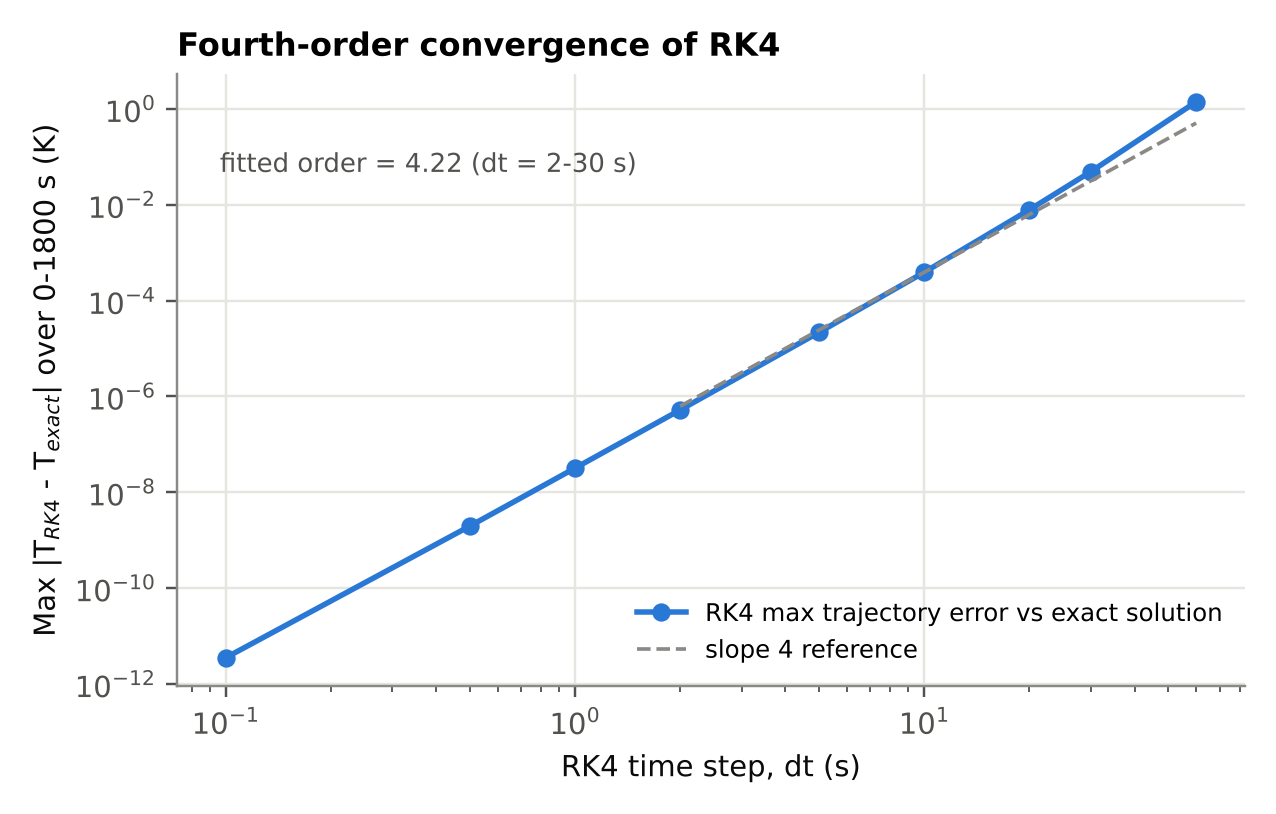
\includegraphics[width=0.72\textwidth]{verification/rk4_convergence.png}
\caption{Maximum trajectory error of RK4 relative to the exact solution. The dashed line has slope 4.}\label{fig:convergence}
\end{figure}

The model was implemented twice, in Python (the reference implementation) and in MATLAB syntax; the MATLAB code was executed in \vOctRuntime, not in MATLAB. Table~\ref{tab:crosscheck} compares them. Deterministic quantities agree to the printed precision of the Octave log. Monte Carlo quantities are two independent estimates, because Octave's Mersenne Twister and NumPy's PCG64 generators draw different samples from the same distributions. They agree within sampling error, and both implementations select the same \vRecRpm\ rpm setting. An automated test suite of 41 tests (Appendix~\ref{app:repro}) covers the model equations, RK4 order and stability, energy closure, the actuator limit, the optimisation logic, the separation of the data sets and the adaptive policy.

\begin{table}[H]
\centering
\caption{Python reference implementation versus the MATLAB-syntax implementation executed in GNU Octave.}\label{tab:crosscheck}
{\small\input{generated/tab_crosscheck.tex}}
\end{table}

\section{Energy-Balance Validation}\label{sec:energy}

Equation~\ref{eq:firstlaw} is evaluated from the RK4 trajectories (Table~\ref{tab:ebal}). The coolant term is integrated with both the trapezoidal rule and Simpson's rule. With the trapezoidal rule the residual at the reference point is \vEBResTrap\ J; with Simpson's rule it falls to \vEBResSimp\ J, a relative residual of \(\vEBRel\). The residual is therefore quadrature error and not a model inconsistency. The balance closes equally well at the recommended setting.

\begin{table}[H]
\centering
\caption{Energy-balance closure over the 1800 s batch (RK4, \(\Delta t = 1\) s).}\label{tab:ebal}
\input{generated/tab_ebal.tex}
\end{table}

\section{Dynamic Simulation Results}

\subsection{Original versus coupled model}
Figure~\ref{fig:orig} compares the two models at the reference point. The coupled liquid ends \vTBaseGap\ K warmer than the original model predicts, and the difference changes the conclusion: the original model says the target is met, while the coupled model says it is not. The jacket coolant does not stay at 300 K; it rises to \vPeakTJBase\ K after about \vPeakTJBaseMin\ min and is still at \vTJBase\ K at the end of the batch.

\begin{figure}[H]
\centering
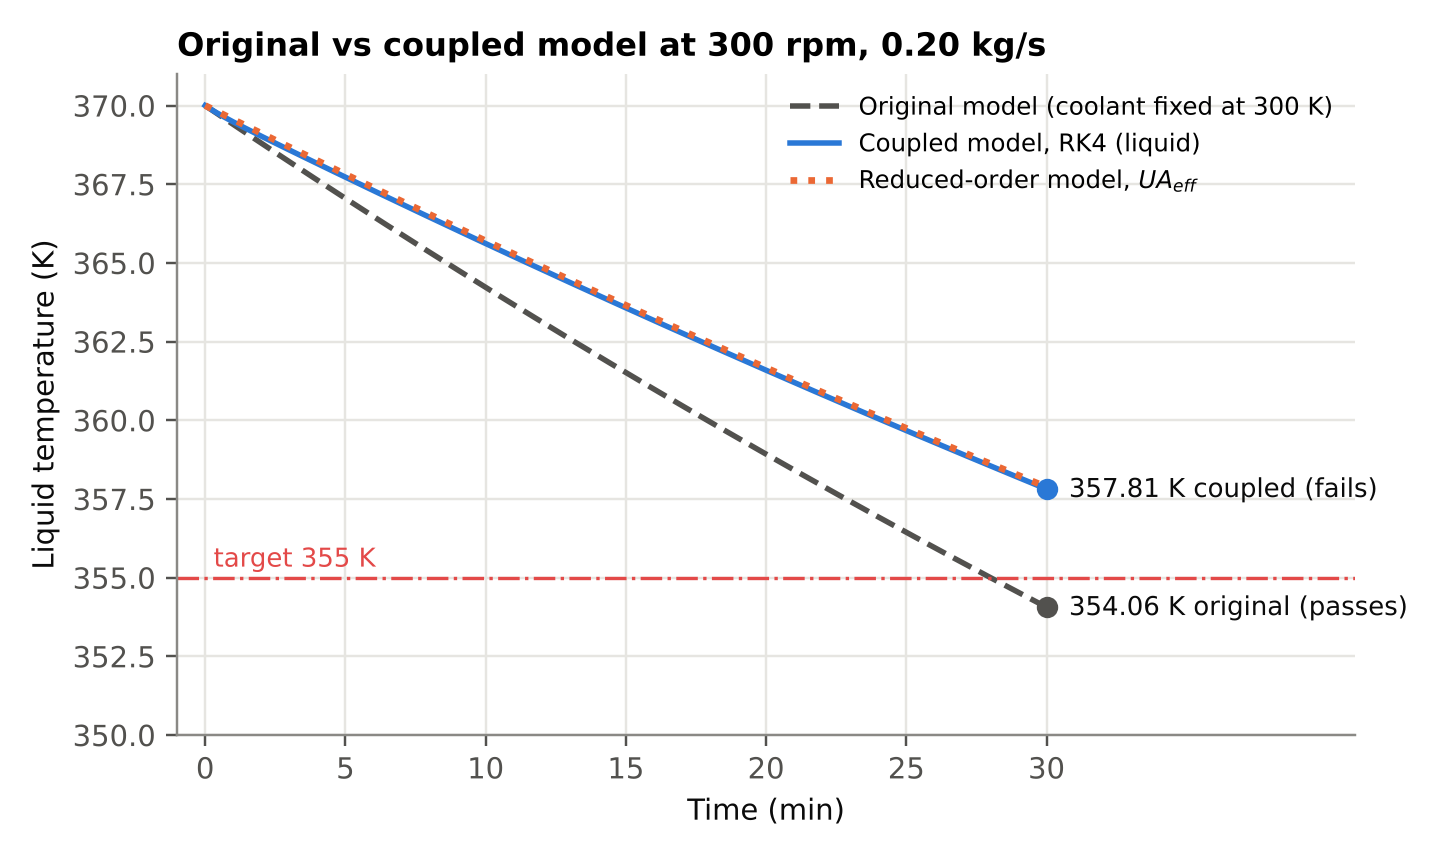
\includegraphics[width=0.78\textwidth]{model_comparison/original_vs_coupled.png}
\caption{Original constant-coolant model, coupled RK4 model and the reduced-order model of Section~\ref{sec:rom} at 300 rpm and 0.20 kg/s.}\label{fig:orig}
\end{figure}

\subsection{Temperature profiles at the main operating points}
Figure~\ref{fig:profiles} and Table~\ref{tab:cases} show the liquid and jacket temperatures for the reference point, the deterministic optimum and the recommended setting. At 0.50 kg/s the coolant heat-capacity rate is 2.5 times higher than at 0.20 kg/s, so the jacket stays within about 11 K of the inlet. In the nominal model the recommended setting reaches 355 K after \vRecTtt\ s (\vRecTttMin\ min) and ends at \vRecTL\ K.

\begin{figure}[H]
\centering
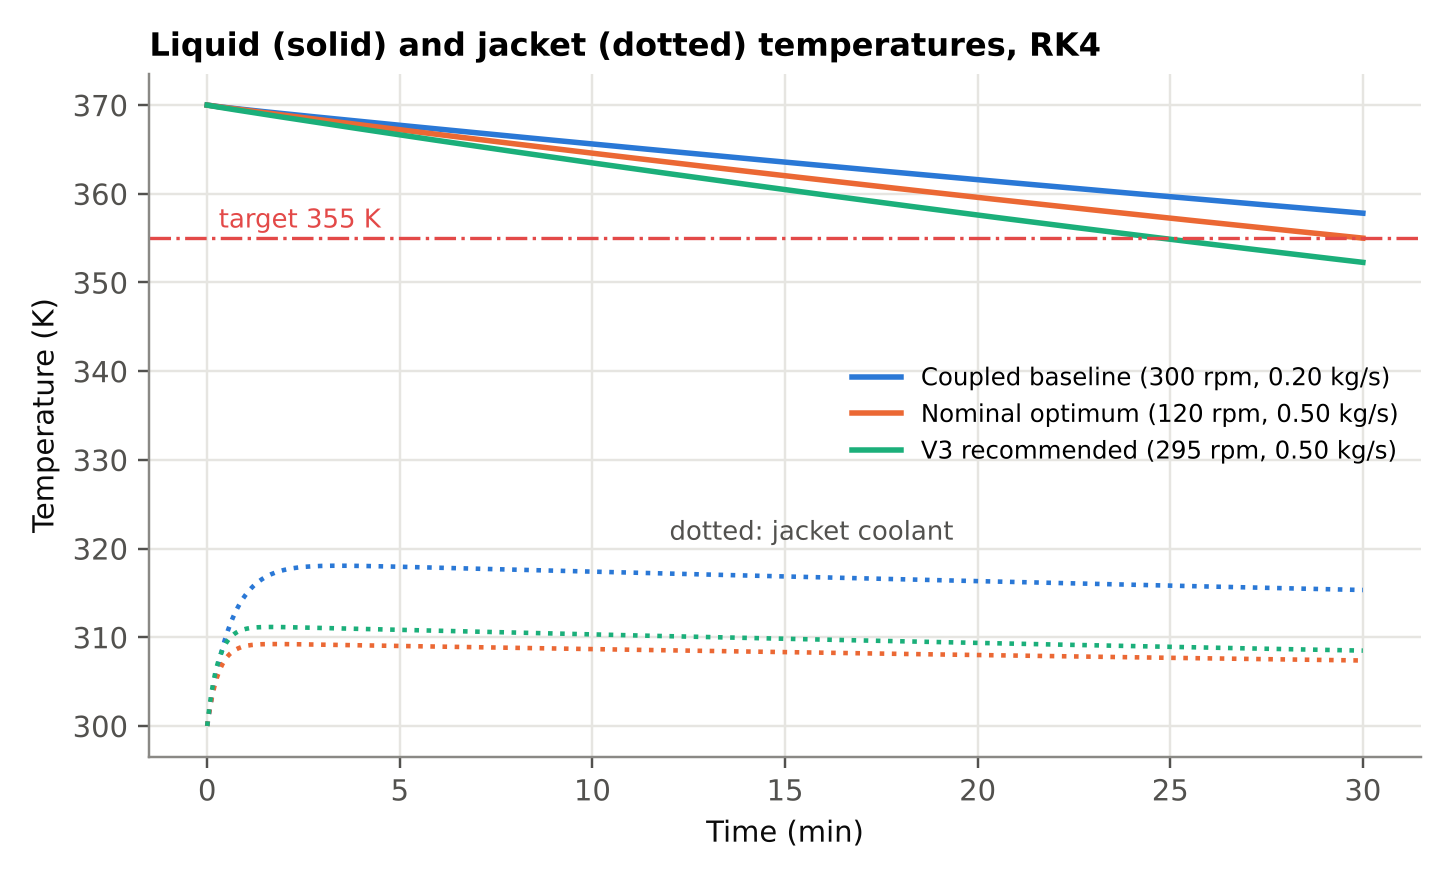
\includegraphics[width=0.78\textwidth]{temperature_profiles/temperature_profiles.png}
\caption{Liquid (solid) and jacket (dotted) temperatures from RK4.}\label{fig:profiles}
\end{figure}

\begin{table}[H]
\centering
\caption{Deterministic comparison of operating points (RK4, \(\Delta t = 1\) s; delivered flow equals commanded flow).}\label{tab:cases}
{\small\setlength{\tabcolsep}{3.5pt}\input{generated/tab_cases.tex}}
\end{table}

\section{Reduced-Order Model}\label{sec:rom}

Because the jacket time constant is much shorter than the batch, the jacket is quasi-steady for most of the batch. Setting \(dT_J/dt = 0\) in Equation~\ref{eq:jacket} gives \(T_J = (UA\,T_L + \mdot C_{p,C} T_{in})/(UA + \mdot C_{p,C})\), and substituting into Equation~\ref{eq:liquid} gives
\begin{equation}
M_LC_{p,L}\frac{dT_L}{dt} = -UA_{eff}\,(T_L - T_{in}),\qquad \frac{1}{UA_{eff}} = \frac{1}{UA} + \frac{1}{\mdot\,C_{p,C}}. \label{eq:uaeff}
\end{equation}
The two resistances act in series: heat must cross the wall (\(1/UA\)) and then be carried away by a coolant stream of finite heat-capacity rate (\(1/\mdot C_{p,C}\)). The liquid then follows a single exponential, \(T_L(t) = T_{in} + (T_0 - T_{in})\exp(-UA_{eff}\,t/M_LC_{p,L})\), the same form as the original model with \(UA\) replaced by \(UA_{eff}\). At the reference point \(UA = 300\) W/K and \(\mdot C_{p,C} = 836\) W/K give \(UA_{eff} = \vUAEffBase\) W/K, which accounts for the whole difference between the original and coupled models.

Setting \(T_L(t_f) = T_{target}\) gives the conductance any design must provide,
\begin{equation}
UA_{eff,req} = \frac{M_LC_{p,L}}{t_f}\,\ln\frac{T_0 - T_{in}}{T_{target} - T_{in}} = \vUAEffReq\ \mathrm{W/K}. \label{eq:uareq}
\end{equation}
Two consequences follow. Because \(UA_{eff} < \mdot C_{p,C}\), the target is unreachable at any agitator speed unless \(\mdot > UA_{eff,req}/C_{p,C} = \vMinFlow\) kg/s. And combining Equations~\ref{eq:closure} and~\ref{eq:uareq} gives the feasibility boundary \(N(\mdot)\) in closed form, which is drawn in Figure~\ref{fig:window}.

Table~\ref{tab:rom} tests the reduced model. Its error is \vRomErrBase\ K at the reference point and \vRomErrRec\ K at the recommended setting. It grows when the jacket time constant is no longer small compared with the batch: with a 100 kg jacket (\(\tau_J/t_f \approx 0.2\)) the error reaches \vRomErrMaxAbs\ K, because the quasi-steady model ignores the heat needed to warm the jacket inventory. The reduced model is therefore a hand-calculation tool for fast jackets, not a replacement for the dynamic model.

\begin{table}[H]
\centering
\caption{Reduced-order (quasi-steady) model versus the full RK4 model at \(t_f = 1800\) s.}\label{tab:rom}
{\small\setlength{\tabcolsep}{3.5pt}\input{generated/tab_rom.tex}}
\end{table}

\section{Local and Global Sensitivity Analysis}

\subsection{Local sensitivity}
Version 1 perturbed each input by \(\pm 20\,\%\), except the initial temperature, which was moved by \(\pm 1\) K. Mixing step sizes makes the ranking reflect the steps rather than the importance of the inputs. Table~\ref{tab:local} therefore also moves each uncertain input by one standard deviation of its assumed distribution, at the reference point and at the recommended setting. On that basis the initial temperature and \(U_{ref}\) have similar local influence, the coolant-flow error is smaller, and the jacket inventory is negligible (Figure~\ref{fig:sens}a). Flow perturbations are saturated at the pump limit. At the recommended setting, which already runs at 0.50 kg/s, an upward flow step is not physically available, so the high-side change is zero by construction; version 2 had evaluated flows above the limit here as well.

\begin{table}[H]
\centering
\caption{Local sensitivity of \(T_L(1800\ \mathrm{s})\) at the reference point.}\label{tab:local}
{\small\input{generated/tab_local.tex}}
\end{table}

\subsection{Global variance-based sensitivity}
Local derivatives do not show how much of the batch-to-batch spread each uncertainty causes. Sobol indices do. For an output \(Y\) and input \(X_i\), the first-order index \(S_i = \mathrm{Var}[E(Y|X_i)]/\mathrm{Var}(Y)\) is the share of variance explained by \(X_i\) alone, and the total-effect index \(S_{T,i} = E[\mathrm{Var}(Y|X_{\sim i})]/\mathrm{Var}(Y)\) includes its interactions. They were estimated with the Saltelli sampling scheme, the Saltelli (2010) estimator for \(S_i\) and the Jansen estimator for \(S_{T,i}\) [5, 6], using \(N = 32{,}768\) base samples (\vSobolRuns\ model runs per design) and 500 bootstrap resamples. The four inputs are independent, so variance-based indices are well defined, but they are conditional on the assumed distributions.

At the recommended setting, \(U_{ref}\) explains \vSobOneU\,\% of the variance of the final temperature, the initial temperature \vSobOneTZero\,\%, the flow-loop error \vSobOneFlow\,\% and the jacket inventory essentially none (Table~\ref{tab:sobol}, Figure~\ref{fig:sens}b). First-order and total indices agree within their intervals, so the inputs act additively. The flow error contributes little at the recommended setting partly because half of the batches are held at the pump limit. The measurement with the greatest value is therefore an estimate of the heat-transfer conductance; the adaptive policy of Section~\ref{sec:adaptive} is built on this.

\begin{table}[H]
\centering
\caption{Sobol indices of \(T_L(1800\ \mathrm{s})\) with 95\,\% bootstrap intervals.}\label{tab:sobol}
{\small\input{generated/tab_sobol.tex}}
\end{table}

\begin{figure}[H]
\centering
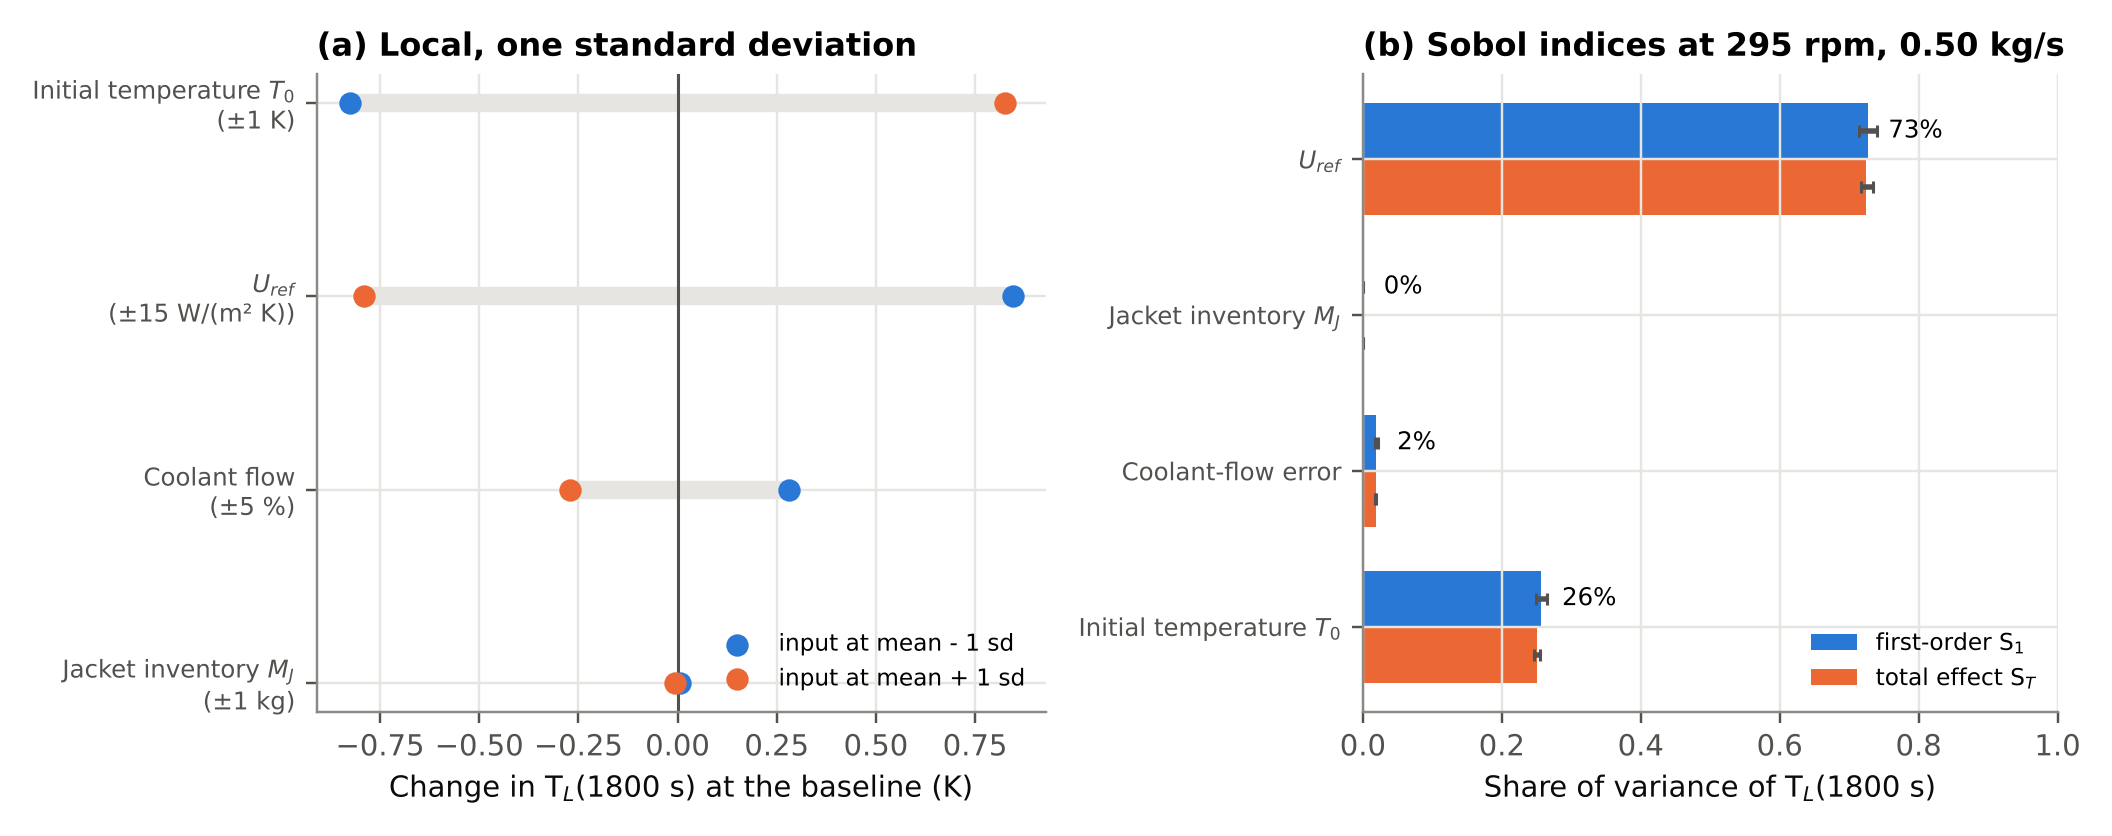
\includegraphics[width=\textwidth]{sensitivity/local_and_sobol.png}
\caption{(a) Local sensitivity at the reference point, each input moved by one standard deviation. (b) Sobol indices at the recommended setting.}\label{fig:sens}
\end{figure}

\section{Deterministic Optimisation}

The deterministic problem is
\begin{equation}
\begin{aligned}
\min_{N,\ \mdot_{cmd}}\ & E(N, \mdot_{cmd})\\
\text{s.t.}\ & T_L(t_f;\,N,\mdot_{cmd}) \le 355\ \mathrm{K},\quad 100 \le N \le 600\ \mathrm{rpm},\quad 0.05 \le \mdot_{cmd} \le 0.50\ \mathrm{kg/s},
\end{aligned} \label{eq:detopt}
\end{equation}
with the delivered flow equal to the commanded flow. Version 1 searched a 5 rpm by 0.005 kg/s grid and found \vGridRpm\ rpm and \vGridM\ kg/s (\vGridE\ kWh). That point is a grid artefact. Since \(T_L(t_f)\) decreases monotonically in both variables, the constraint is active at the optimum. The speed on the constraint is found for each flow with Brent's method, and the energy along the constraint is minimised with a bounded scalar search. The optimum lies on the flow bound, at \vNomRpm\ rpm and 0.50 kg/s, with \vNomEFour\ kWh per batch. Both the cooling constraint and the pump limit are active: coolant flow is the cheaper lever, because agitator power grows with \(N^3\) while \(U\) grows only with \(N^{0.25}\). Figure~\ref{fig:window} maps the energy over the operating window, together with the simulated and closed-form feasibility boundaries.

\begin{figure}[H]
\centering
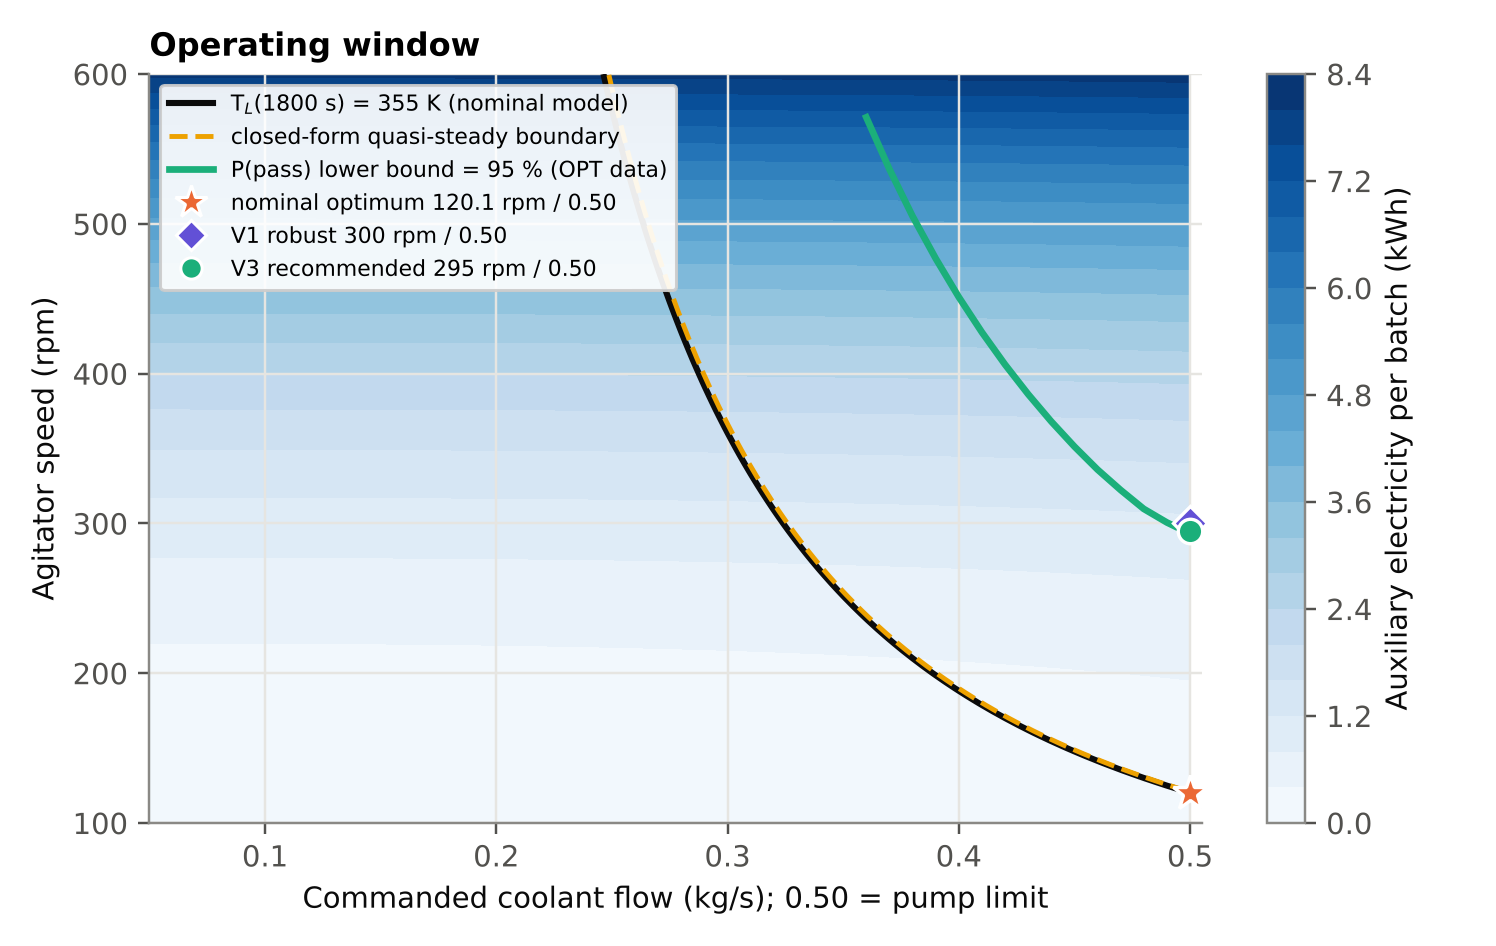
\includegraphics[width=0.8\textwidth]{optimization/operating_window.png}
\caption{Operating window. Shading: auxiliary electricity per batch. Black: nominal 355 K boundary; yellow dashed: closed-form boundary from Equations~\ref{eq:closure} and~\ref{eq:uareq}; green: 95\,\% reliability boundary with the lower-bound rule on the optimisation data. Feasible settings lie above and to the right of each curve.}\label{fig:window}
\end{figure}

The nominal optimum sits exactly on the constraint, so roughly half of all simulated batches miss the target: only \vNomPass\,\% pass on the independent validation set. A design rule is needed that includes reliability explicitly.

\section{Monte Carlo Uncertainty Analysis}\label{sec:mc}

\subsection{Uncertainty model and data sets}
Four inputs are uncertain and independent: \(U_{ref} \sim \mathcal N(150, 15^2)\) W/(m\textsuperscript{2}K), \(M_J \sim \mathcal N(10, 1^2)\) kg, the flow-loop error \(z \sim \mathcal N(0,1)\) in Equation~\ref{eq:actuator}, and \(T_0 \sim \mathcal N(370, 1^2)\) K. These spreads are assumptions, not measured statistics. Each Monte Carlo data set has a fixed seed and a single purpose (Table~\ref{tab:datasets}). Designs are chosen on OPT, the adaptive policy is calibrated and configured on CAL, and every reported reliability comes from VAL, a set that played no part in any choice and was evaluated once per design. VAL2 is held in reserve for a design that fails VAL and has to be modified by a pre-declared rule; neither the fixed setting nor the adaptive policy needed it. The validation seeds are new for this release. The seeds examined during development (20261110, 20261111 and 20261115) were retired, so no validation number reported here was seen before the final run. STRESS is used only for stress tests, never for selection.

\begin{table}[H]
\centering
\caption{Monte Carlo data sets. Each seed is fixed and each set has one purpose.}\label{tab:datasets}
{\small\input{generated/tab_datasets.tex}}
\end{table}

\subsection{Statistics}
For \(k\) passing batches out of \(n\), the pass fraction \(\hat p = k/n\) is reported with the Wilson score interval [7],
\begin{equation}
\frac{\hat p + \frac{z^2}{2n} \pm z\sqrt{\frac{\hat p(1-\hat p)}{n} + \frac{z^2}{4n^2}}}{1 + \frac{z^2}{n}}, \label{eq:wilson}
\end{equation}
with \(z = 1.960\) for the two-sided 95\,\% interval and \(z = 1.645\) for the one-sided 95\,\% lower bound. Figure~\ref{fig:mc}b shows that a single estimate near 95\,\% based on 10{,}000 batches has a two-sided interval of about \(\pm0.4\) percentage points, which is why the validation sets in this version contain 200{,}000 batches.

\subsection{Earlier designs under the corrected model}
Table~\ref{tab:designs} re-evaluates the earlier recommendations under the saturated actuator and actual-flow pump energy. Removing the impossible high-flow batches lowers every design's reliability. The version-2 recommendation of 285 rpm falls to \vVTwoRecPass\,\% (lower bound \vVTwoRecLB\,\%) and no longer meets the 95\,\% requirement. Version 1's 300 rpm setting still passes (\vVOneRobPass\,\%) but uses \vVOneRobE\ kWh. Figure~\ref{fig:actuator} shows the delivered-flow distribution and the resulting pass rates.

\begin{table}[H]
\centering
\caption{Designs evaluated on the independent validation set under the corrected model. ``Rule met'': one-sided 95\,\% lower bound \(\ge\) 95\,\%.}\label{tab:designs}
{\small\input{generated/tab_designs.tex}}
\end{table}

\begin{figure}[H]
\centering
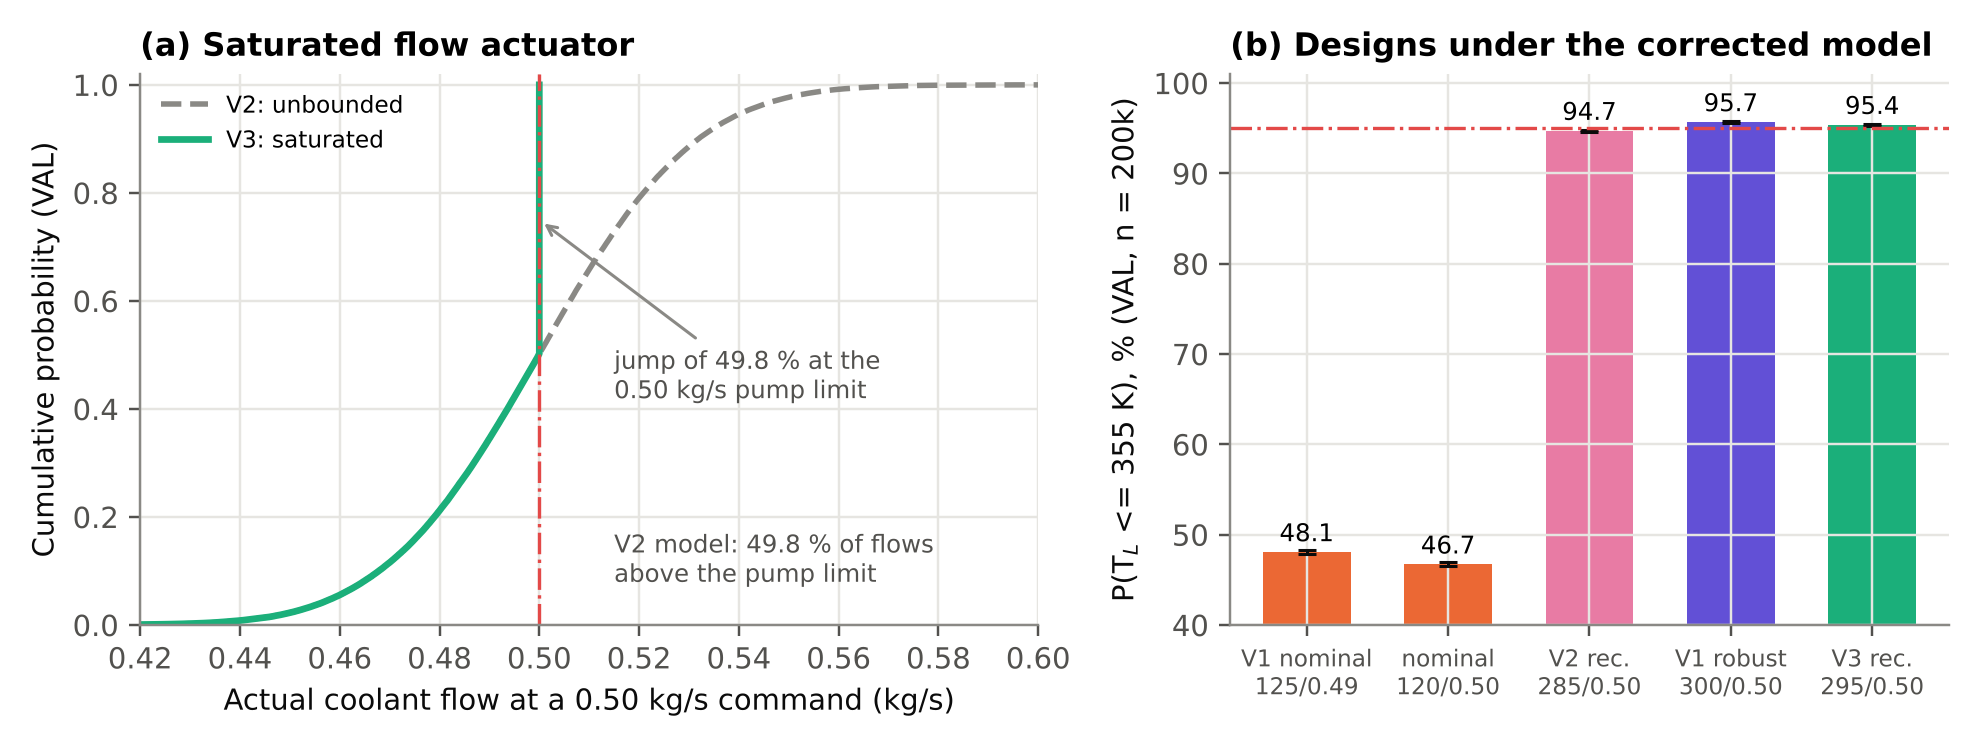
\includegraphics[width=\textwidth]{monte_carlo/flow_actuator_and_designs.png}
\caption{(a) Cumulative distribution of delivered coolant flow at a 0.50 kg/s command: version 2's unbounded error model against the saturated actuator. (b) Pass probability of the main designs with 95\,\% Wilson intervals.}\label{fig:actuator}
\end{figure}

\begin{figure}[H]
\centering
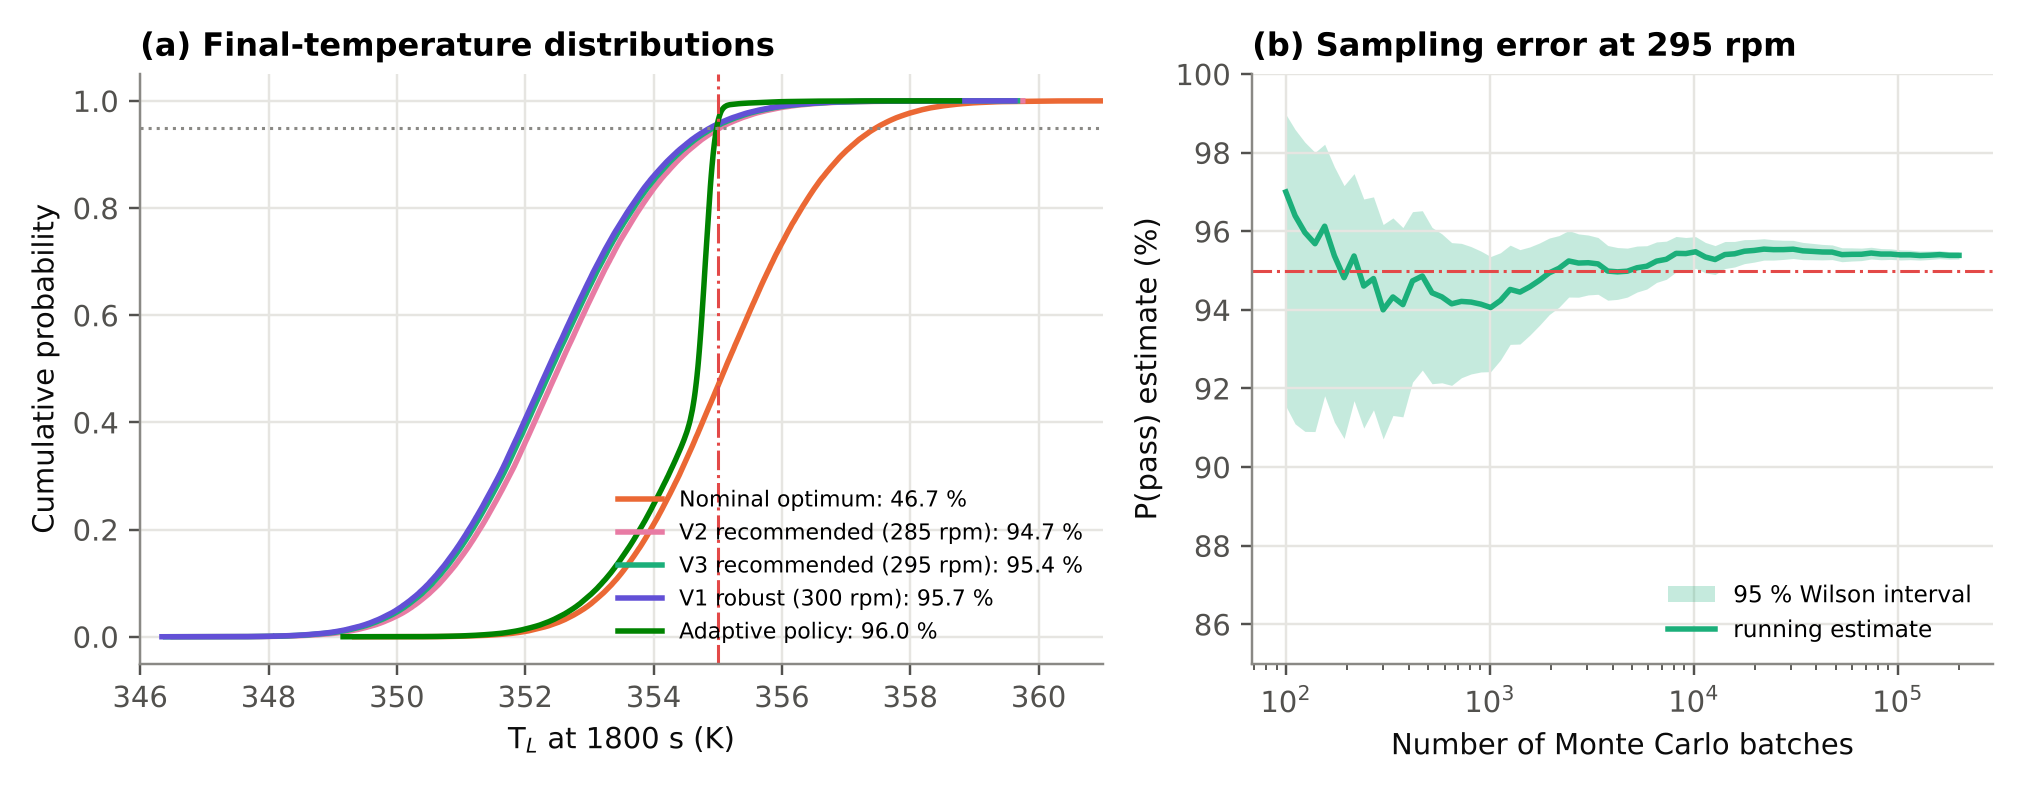
\includegraphics[width=\textwidth]{monte_carlo/final_temperature_and_convergence.png}
\caption{(a) Cumulative distributions of \(T_L(1800\ \mathrm{s})\) on the independent sets; the pass probability is read where each curve crosses 355 K. (b) Running estimate of the pass probability at the recommended setting with its 95\,\% Wilson interval.}\label{fig:mc}
\end{figure}

\section{Reliability-Based Optimisation}

\subsection{Chance-constrained formulation}
The design problem with uncertainty is
\begin{equation}
\min_{N,\ \mdot_{cmd}}\ \mathbb{E}\left[E(N, \mdot)\right]\quad \text{s.t.}\quad \Pr\left[T_L(t_f) \le 355\ \mathrm{K}\right] \ge \alpha = 0.95, \label{eq:cc}
\end{equation}
within the same bounds, with \(\mdot\) the delivered flow of Equation~\ref{eq:actuator}. The objective is the expected energy, because the pump energy now varies with the delivered flow. The chance constraint is replaced by a sample-average approximation on the OPT set [8], with a margin for the sampling error of that set: the design must satisfy
\begin{equation}
\mathrm{LB}_{95}\left(\hat p_{\mathrm{OPT}}\right) \ge \alpha \quad\Longleftrightarrow\quad \hat p_{\mathrm{OPT}} \ge \vPReqOpt\,\% \ \text{for } n = \vNOpt, \label{eq:saa}
\end{equation}
where \(\mathrm{LB}_{95}\) is the one-sided Wilson lower bound. All candidate settings are evaluated on the same samples (common random numbers). For a fixed sample, \(T_L(t_f)\) decreases monotonically with speed, so the pass fraction is non-decreasing in \(N\). The lowest speed that meets Equation~\ref{eq:saa} is therefore found exactly by bisection at each commanded flow on a 0.005 kg/s grid, and the expected energy is minimised over flow.

\subsection{Selection and validation protocol}
The protocol was fixed before validation: (i) solve Equation~\ref{eq:cc} on OPT; (ii) round the speed \emph{up} to the next 5 rpm to give a practical setpoint, re-checking Equation~\ref{eq:saa} on OPT only; (iii) validate once on VAL and accept if the one-sided 95\,\% lower bound is at least 95\,\%; (iv) only if the design fails, add 5 rpm and validate on the untouched VAL2 set. Table~\ref{tab:audit} records every stage. The continuous optimum is \vCCRpm\ rpm at 0.50 kg/s. Rounding gives \vRecRpm\ rpm, and on VAL the setting passes in \vRecPass\,\% of batches (95\,\% CI \vRecLo--\vRecHi\,\%, one-sided lower bound \vRecLB\,\%). It is \vRecValStage. The independent Octave implementation, with different random samples, finds a continuous optimum of \vOctCCRpm\ rpm, rounds to the same \vRecRpm\ rpm and validates it at \vOctRecPass\,\%.

\begin{table}[H]
\centering
\caption{Audit trail of the recommended fixed setting.}\label{tab:audit}
{\small\input{generated/tab_audit.tex}}
\end{table}

\textbf{Recommended fixed operating point: \vRecRpm\ rpm agitator speed, \vRecM\ kg/s commanded coolant flow.} Expected auxiliary electricity is \vRecE\ kWh per batch (agitator \vRecAgW\ W; pump \vRecPumpW\ W at the commanded flow, less on average at the delivered flow). The setting uses \vRecVsVOne\,\% less energy than version 1's 300 rpm choice for the same requirement. The saving is small: correcting the flow model has used up most of the margin that version 2 appeared to find.

\subsection{Reliability--energy frontier}
Repeating the procedure for \(\alpha\) from 50\,\% to 99\,\% gives the frontier in Table~\ref{tab:frontier} and Figure~\ref{fig:frontier}. Every point is validated on VAL, and \vFrAllAccepted\ of them meet their own lower-bound requirement. Every optimum lies at the pump limit. Raising the requirement from 50\,\% to 90\,\% multiplies the energy by \vFrRatioA, and going from 90\,\% to 99\,\% multiplies it by a further \vFrRatioB\ (\vFrNinetyNineE\ kWh at \vFrNinetyNineRpm\ rpm). Each extra percentage point of reliability costs more energy than the last, because agitator power grows with the cube of speed while the heat-transfer coefficient grows only with its fourth root.

\begin{table}[H]
\centering
\caption{Reliability--energy frontier (optimised on OPT, validated on VAL).}\label{tab:frontier}
{\small\input{generated/tab_frontier.tex}}
\end{table}

\begin{figure}[H]
\centering
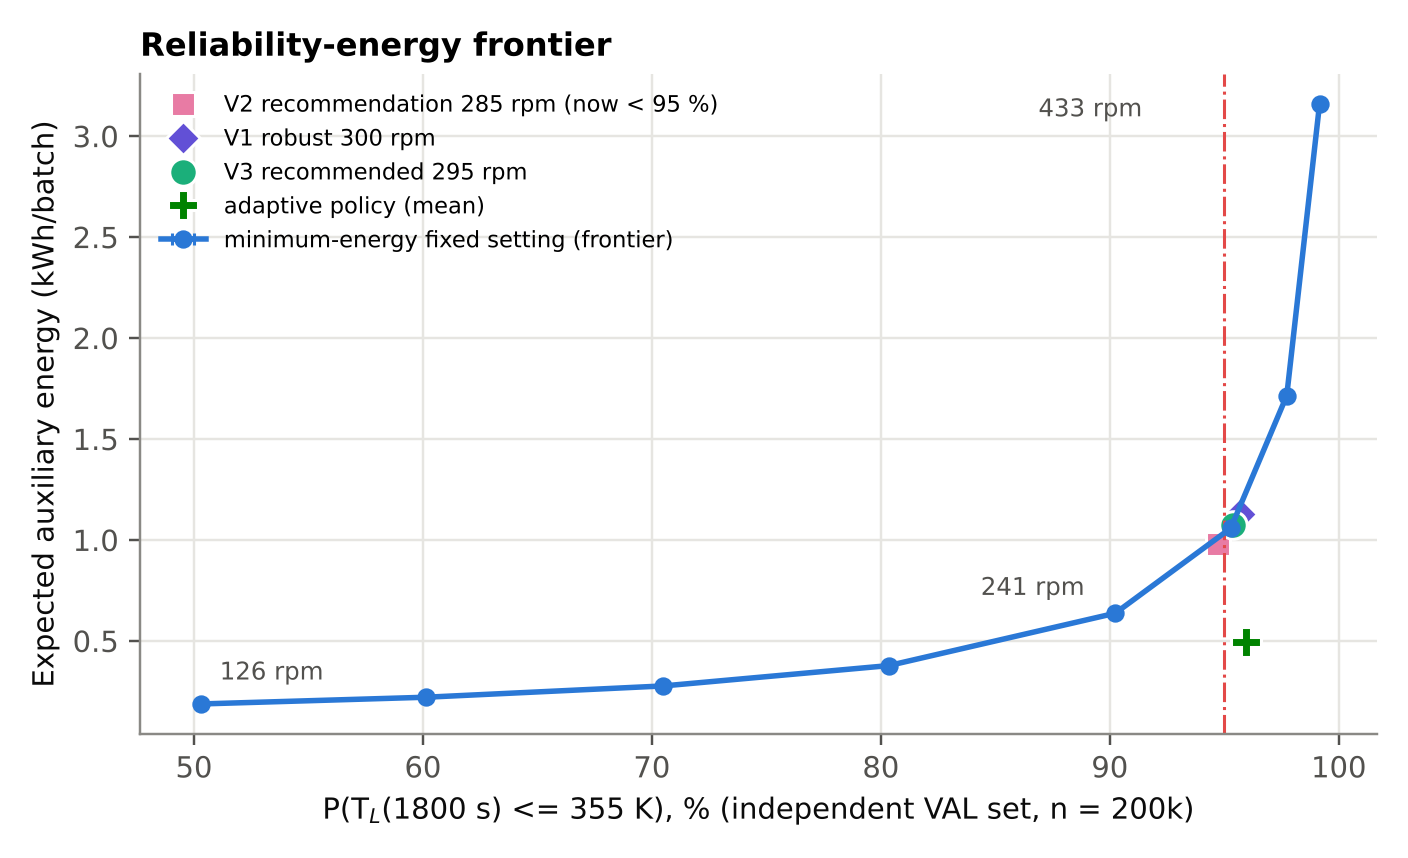
\includegraphics[width=0.8\textwidth]{optimization/reliability_energy_frontier.png}
\caption{Expected auxiliary electricity needed for each pass probability, with the earlier designs, the recommended setting and the adaptive policy. Horizontal bars are 95\,\% Wilson intervals.}\label{fig:frontier}
\end{figure}

\subsection{Value of more pump capacity (hypothetical)}
Since every reliable design sits on the pump limit, the value of more pump capacity was estimated by re-solving Equation~\ref{eq:cc} with a higher limit (Table~\ref{tab:relax}). This is a hypothetical equipment change, and the pressure drop is extrapolated with the assumed quadratic law. A limit of 0.55 kg/s would lower the 95\,\% design energy by about \vRelaxFiftyFiveCut\,\% (to \vRelaxFiftyFiveE\ kWh). Pump and jacket hydraulics, not a larger agitator drive, are therefore what an equipment study should examine first.

\begin{table}[H]
\centering
\caption{Minimum-energy 95\,\% design for a hypothetical higher pump limit (\(\Delta P \propto \mdot^2\), OPT data).}\label{tab:relax}
{\small\input{generated/tab_relax.tex}}
\end{table}

\section{Adaptive Operating Strategy}\label{sec:adaptive}

\subsection{Policy}
A fixed setting must be sized for the worst plausible batch, so most batches are over-agitated. Since about three quarters of the outcome variance comes from \(U_{ref}\), measuring the heat-transfer conductance early in each batch should let the agitation be set for the batch actually being cooled. The simulated policy has two phases.
\begin{enumerate}[leftmargin=*]
\item \textbf{Phase 1} (\(0 \le t < t_{obs}\)): run at speed \(N_1\) with the commanded flow at its maximum, and log \(T_L\) and \(T_J\) every 10 s with Gaussian sensor noise of standard deviation \(\sigma = 0.1\) K (an assumption).
\item \textbf{Estimation} (soft sensor, from 120 s, after the jacket transient): straight-line fits to \(T_L(t)\) and \(T_J(t)\) give
\begin{equation}
\hat Q = -M_LC_{p,L}\,\widehat{\frac{dT_L}{dt}},\qquad \widehat{UA} = \frac{\hat Q}{\bar T_L - \bar T_J},\qquad \widehat{\mdot C_p} = \frac{\hat Q - M_JC_{p,C}\,\widehat{dT_J/dt}}{\bar T_J - T_{in}}. \label{eq:softsensor}
\end{equation}
Only the two temperature sensors that a jacketed vessel normally has are used.
\item \textbf{Phase 2} (\(t_{obs} \le t \le t_f\)): choose the lowest speed \(N_2 \in [100, 600]\) rpm whose prediction from the estimated state, with \(U\) scaled by \((N_2/N_1)^{e_N}\) and Equation~\ref{eq:exact}, reaches \(355\ \mathrm{K} - \delta\) by \(t_f\). If no speed suffices, the batch runs at 600 rpm and is counted as speed-capped.
\end{enumerate}
The energy is Equation~\ref{eq:energy} with piecewise-constant agitator power and the pump at the delivered flow.

\subsection{Calibration, selection and validation}
For each of twelve combinations of \(N_1 \in \{120, 160, 200, 240\}\) rpm and \(t_{obs} \in \{300, 600, 900\}\) s, the margin \(\delta\) was found by bisection on the CAL set as the smallest value meeting the same lower-bound rule as the fixed design. It was then rounded \emph{up} to the next 0.05 K. This practical rounding is the counterpart of rounding the fixed speed up to 5 rpm, and it is written into the code before any validation run, so it uses CAL data only. The configuration with the lowest mean energy on CAL at the rounded margin was selected (Table~\ref{tab:adscan}): \(N_1 = \vAdRpmOne\) rpm for \(t_{obs} = \vAdTobs\) s, with a calibrated margin of \vAdDeltaCal\ K rounded to \(\delta = \vAdDelta\) K.

\begin{table}[H]
\centering
\caption{Adaptive-policy configurations on the calibration set (selected configuration in bold).}\label{tab:adscan}
{\small\input{generated/tab_adaptive_scan.tex}}
\end{table}

The selected policy was then validated once on VAL with the same acceptance rule as the fixed setting (Table~\ref{tab:adval}). It passes in \vAdPass\,\% of batches (95\,\% CI \vAdLo--\vAdHi\,\%, one-sided lower bound \vAdLB\,\%), so it is \vAdStage. Rounding the margin up matters here. A margin tuned exactly to the threshold on a finite calibration set tends to overstate reliability on new data, the optimiser's curse [10]. In the development runs the unrounded margin validated on one generator but fell just short of the rule on the other. The independent Octave implementation calibrates its own margin on its own samples, applies the same rounding rule and validates at \vOctAdPass\,\% (lower bound \vOctAdLB\,\%).

\begin{table}[H]
\centering
\caption{Validation of the adaptive policy (independent set, used once).}\label{tab:adval}
{\small\setlength{\tabcolsep}{3.5pt}\input{generated/tab_adaptive_val.tex}}
\end{table}

\subsection{Performance}
The soft sensor identifies \(UA\) with a relative error of \vAdUAErr\,\% (one standard deviation) after \vAdTobsMin\ minutes. The validated policy uses a mean of \vAdMeanE\ kWh per batch (median \vAdMedE\ kWh), \vAdSave\,\% less than the fixed \vRecRpm\ rpm setting at a comparable reliability. Most batches finish at a modest speed (median \(N_2 = \vAdMedRpm\) rpm). The energy distribution has a long tail, however: the 95th percentile is \vAdPNFE\ kWh, the 99th percentile \vAdPNNE\ kWh, and \vAdCap\,\% of batches need more than 600 rpm and are speed-capped, at about \vAdCapEnergy\ kWh each (Figure~\ref{fig:adaptive}). Version 2's figure labelled all batches above 3.2 kWh as speed-capped; these are different quantities. In version 3, \vAdFracAboveThree\,\% of batches use more than 3.2 kWh, of which \vAdCap\ percentage points are speed-capped. The figure now shows the capped batches separately.

\begin{figure}[H]
\centering
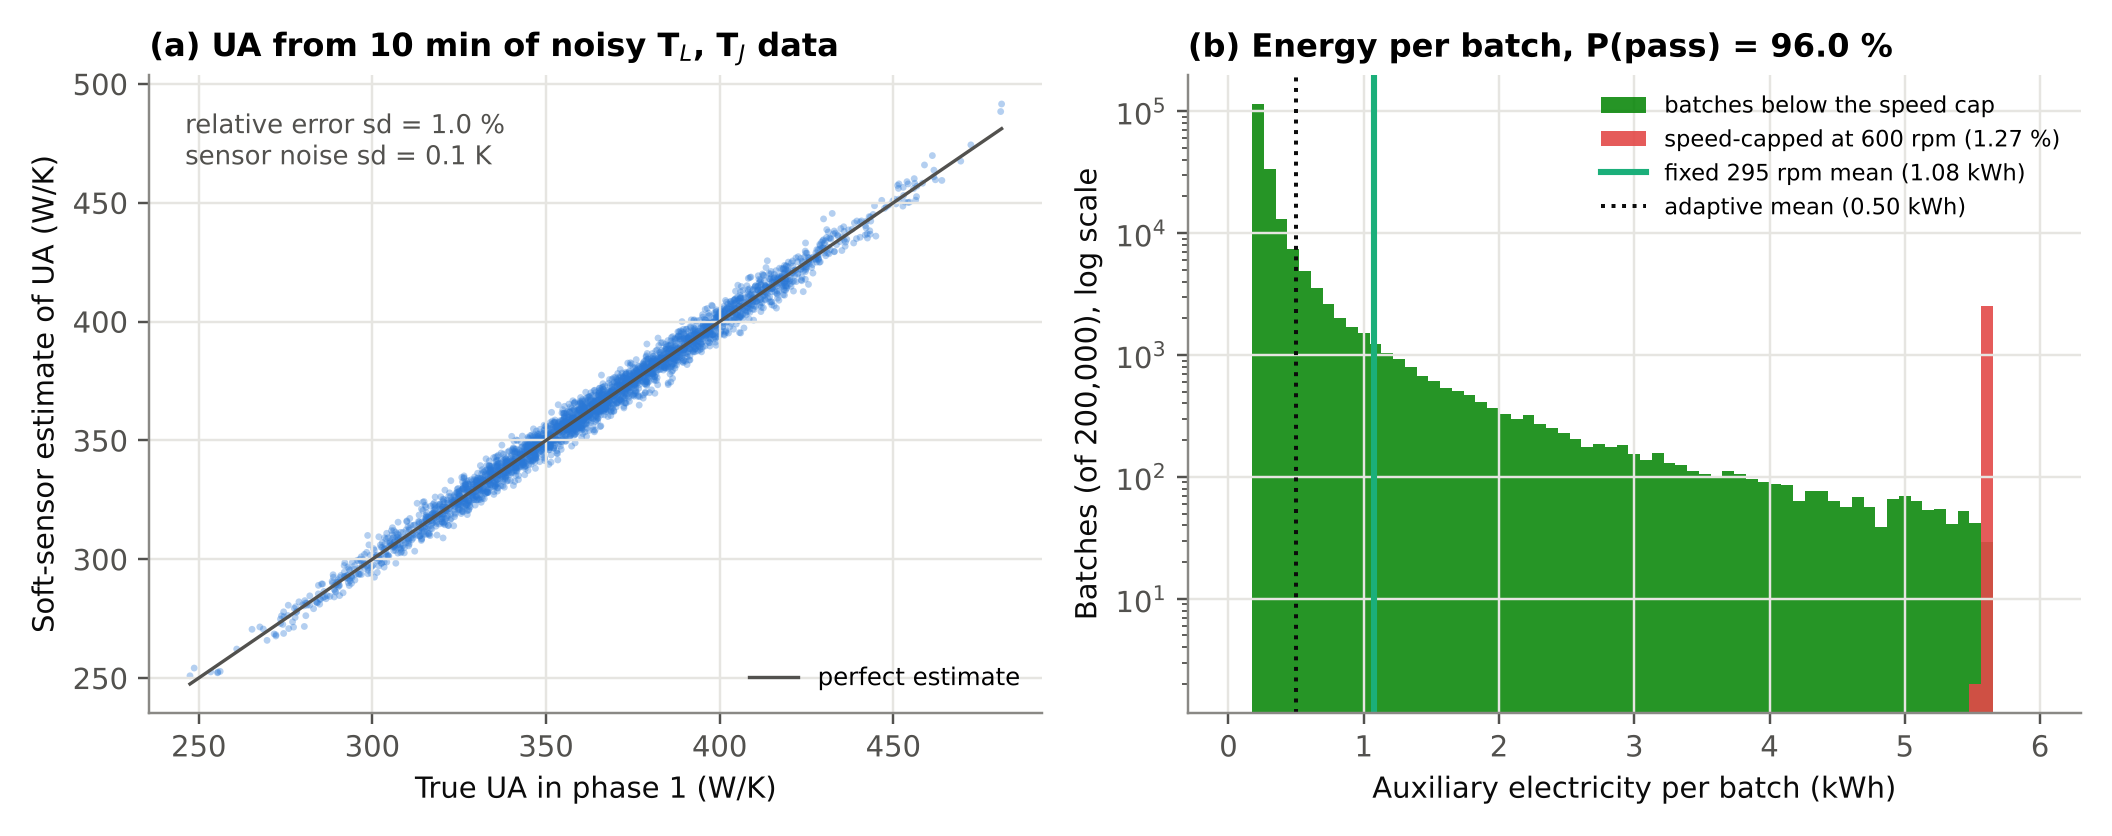
\includegraphics[width=\textwidth]{adaptive_policy/adaptive_policy.png}
\caption{(a) Soft-sensor estimate of \(UA\) against the true value for 3000 validation batches. (b) Energy per batch under the adaptive policy (log scale), with speed-capped batches in red.}\label{fig:adaptive}
\end{figure}

\subsection{Robustness}
Table~\ref{tab:adrob} tests the policy on the STRESS set. With noisier sensors the re-calibrated margin grows and the energy advantage shrinks: at \(\sigma = 0.5\) K the mean energy rises to \vRobHalfE\ kWh. More importantly, the policy extrapolates the effect of a speed change through \(e_N\). If the planner assumes \(e_N = 0.10\) or \(0.40\) while the plant follows 0.25, reliability falls to \vRobLowEN\,\% or \vRobHighEN\,\%. The policy is therefore worth deploying only after the speed dependence of \(U\) has been identified, for example from a speed step test using the same estimator. It has not been tested experimentally.

\begin{table}[H]
\centering
\caption{Adaptive-policy robustness (STRESS set; \(\delta\) re-calibrated on CAL for each sensor-noise level and rounded up to 0.05 K).}\label{tab:adrob}
{\small\input{generated/tab_adaptive_robust.tex}}
\end{table}

\section{Model-Form Uncertainty and Stress Testing}\label{sec:modelform}

\subsection{Why structural uncertainty is treated differently}
Uncertainty in a parameter value, such as \(U_{ref}\), can be described by a distribution and propagated by Monte Carlo sampling. Uncertainty in the \emph{form} of the model, such as the exponents of Equation~\ref{eq:closure} or the mixing pattern in the jacket, is different. There is no data set from which to estimate a distribution, and assigning one arbitrarily would turn an untested assumption into an apparently precise probability. Model form is therefore examined with structured scenarios, and the conclusions are stated as conditional on the closure being correct.

\subsection{Exponents of the heat-transfer closure}
The exponents can be bounded physically. Writing \(1/U = 1/h_i + R_w + 1/h_o\), with the agitated-side film coefficient \(h_i \propto N^{2/3}\) (the Chilton--Drew--Jebens form [9]) and the coolant-side coefficient \(h_o \propto \mdot^{b}\), with \(b \le 0.8\) for turbulent forced convection [1], the local elasticities of \(U\) are
\begin{equation}
e_N = \tfrac{2}{3}\,\frac{1/h_i}{1/U},\qquad e_M = b\,\frac{1/h_o}{1/U}\quad\Longrightarrow\quad \frac{e_N}{2/3} + \frac{e_M}{0.8} \le 1, \label{eq:admissible}
\end{equation}
because the resistance shares cannot sum to more than one. The nominal exponents imply an inside-film share of \vFIn, a coolant-film share of \vFCo\ and a wall-plus-fouling share of \vFWall, so they are admissible. Three scenarios keep the ratio of inside to coolant resistance and vary the wall-plus-fouling share: \emph{weak scaling} (share 0.60, as for a heavily fouled wall: \(e_N = \vWeakEN\), \(e_M = \vWeakEM\)), the nominal closure, and \emph{strong scaling} (no wall or fouling resistance: \(e_N = \vStrongEN\), \(e_M = \vStrongEM\)). \(U_{ref}\) at the reference point is unchanged in every scenario.

\begin{table}[H]
\centering
\caption{Closure scenarios (STRESS set). ``Fixed'': the recommended \vRecRpm\ rpm setting. ``Adaptive'': the validated policy, planning with the nominal closure. ``Re-opt.\ \(E\)'': minimum expected energy of a 95\,\% fixed design if the scenario were known.}\label{tab:scenarios}
{\small\input{generated/tab_scenarios.tex}}
\end{table}

The results (Table~\ref{tab:scenarios}, Figure~\ref{fig:modelform}) show that model form matters more than any of the parameter uncertainties. Under weak scaling the recommended setting passes only \vWeakFixed\,\% of batches and no fixed setting within the bounds reaches 95\,\% (re-optimised energy: \vWeakReE). Under strong scaling it passes \vStrongFixed\,\%, and a re-optimised design would need only \vStrongReE\ kWh. Over the full grid of admissible exponents, the recommended setting falls below 95\,\% in \vGridFracAdmFail\,\% of combinations, mostly those with a weaker flow dependence. The adaptive policy is \emph{more} sensitive to the closure than the fixed setting, because it relies on \(e_N\) to extrapolate from \(N_1\) to \(N_2\): \vWeakAd\,\% under weak and \vStrongAd\,\% under strong scaling. A safety margin on the operating point does not protect against a wrong closure; calibration does. The first experiments should therefore be a coolant-flow step test and an agitator-speed step test, from which \(U_{ref}\), \(e_M\) and \(e_N\) can be fitted with the same soft-sensor equations.

\begin{figure}[H]
\centering
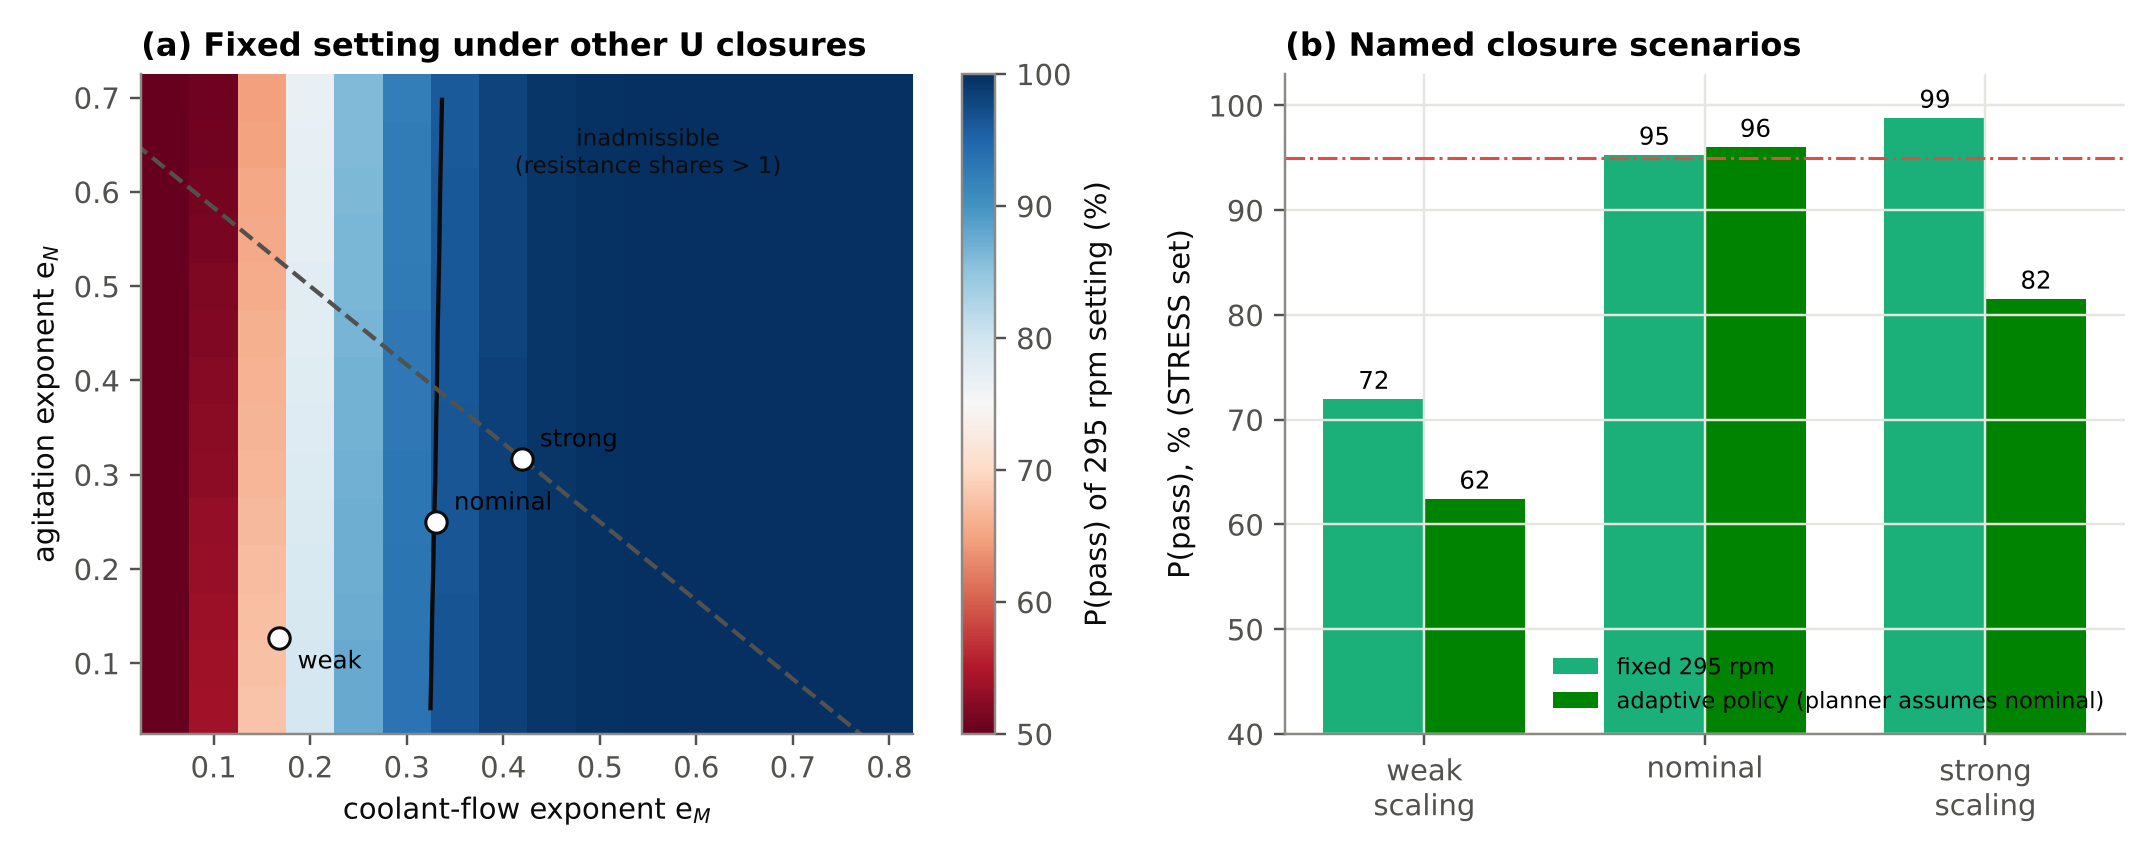
\includegraphics[width=\textwidth]{model_form/closure_stress_test.png}
\caption{(a) Pass probability of the recommended setting over the exponent plane; the solid line is the 95\,\% contour, and settings above and to the right of the dashed line are inadmissible by Equation~\ref{eq:admissible}. (b) Fixed setting and adaptive policy under the three named scenarios.}\label{fig:modelform}
\end{figure}

\subsection{Jacket flow pattern}
The base model treats the jacket as one well-mixed cell. A real jacket lies somewhere between that and plug flow. Dividing the jacket into \(n\) equal well-mixed cells in series, integrated with a vectorised RK4, spans that range (Table~\ref{tab:jacket}). At the quasi-steady limit, plug flow has the effectiveness \(1 - e^{-NTU}\), compared with \(NTU/(1+NTU)\) for a mixed jacket, which is always lower. A plug-flow jacket would therefore raise the effective conductance by about \vJetGainBase\,\% at the reference point and \vJetGainRec\,\% at the recommended setting. The 20-cell model ends \vJetRecTwenty\ K instead of \vJetRecOne\ K at the recommended setting, and with 10 cells the recommended setting passes \vJetPassTen\,\% of STRESS batches instead of \vJetPassOne\,\%. The well-mixed assumption is therefore the conservative limit, and the recommendation is on the safe side with respect to jacket mixing.

\begin{table}[H]
\centering
\caption{Final liquid temperature with the jacket divided into well-mixed cells in series (RK4).}\label{tab:jacket}
{\small\input{generated/tab_jacket.tex}}
\end{table}

\subsection{Jacket thermal inventory (isolated study)}
Changing only \(M_J\) from 5 to 100 kg, with all other parameters fixed, changes \(T_L(1800\ \mathrm{s})\) at the recommended setting by \vMJSpread\ K (Table~\ref{tab:inventory}). Even at 100 kg the jacket time constant (\vMJTauHundred\ s) is much shorter than the batch. This is an \emph{isolated thermal-inventory} sensitivity, and it does not show that jacket geometry is unimportant. A different gap or flow path would also change the coolant velocity, the pressure drop and the coolant-side coefficient (Table~\ref{tab:equipment}), and through them \(U\), \(e_M\) and the pump energy, none of which are held fixed in a real redesign.

\begin{table}[H]
\centering
\caption{Isolated effect of the jacket thermal inventory.}\label{tab:inventory}
{\small\input{generated/tab_inventory.tex}}
\end{table}

\section{Engineering Interpretation and Recommendations}

\begin{enumerate}[leftmargin=*]
\item \textbf{Model the coolant side.} The jacket is not an infinite sink. The coolant heat-capacity rate is a series resistance that reverses the pass/fail decision at the reference point, and Equation~\ref{eq:uaeff} is a hand check that any process engineer can apply.
\item \textbf{Use the maximum coolant flow, then add agitation.} Every optimum, deterministic or reliability-constrained, sits at the pump limit. The flow is the cheap lever, and pump capacity is the constraint worth studying.
\item \textbf{Specify reliability, not only feasibility.} A setting that just meets 355 K in the nominal model fails about half the time. For 95\,\% reliability under the stated assumptions, run at \vRecRpm\ rpm with \vRecM\ kg/s commanded (\vRecE\ kWh per batch), and quote that reliability with its confidence interval and the uncertainty model behind it.
\item \textbf{Calibrate before optimising further.} The heat-transfer closure dominates both the parameter uncertainty (through \(U_{ref}\)) and the structural uncertainty (through \(e_M\) and \(e_N\)). Coolant-flow and agitator-speed step tests should come first.
\item \textbf{Adaptive operation is promising but conditional.} In simulation it halves the expected energy at the same reliability, but only with sensors of about 0.1--0.2 K, a variable-speed drive and an identified speed exponent. It should be tested at pilot scale before any claim of real savings.
\end{enumerate}

\section{Limitations and Future Work}

\begin{itemize}[leftmargin=*]
\item The model is lumped: perfectly mixed liquid, a single overall coefficient, no wall heat capacity, no heat loss, evaporation or reaction heat. A multi-cell jacket with a hydraulic model, and wall capacitance, are the natural next steps.
\item The heat-transfer closure, power number, efficiencies, loop pressure drop and pump limit are assumed screening values. No experimental or vendor data have been used.
\item The input distributions are assumed independent and normal. Plant data may show skewed, correlated or drifting behaviour, and the reliability figures would then need to be re-estimated.
\item The energy objective covers agitator and pump electricity only. Chiller or cooling-tower energy and water cost would favour lower coolant flows and could move the optimum.
\item The adaptive policy assumes a variable-speed drive, 10 s logging and a known speed exponent; the 600 rpm cap is a modelling bound.
\item The 355 K and 1800 s target is illustrative. The methods transfer to other targets; the specific numbers do not.
\end{itemize}

\section{Conclusion}

The ESC113M cooling problem has been extended from a single exponential decay to a verified two-state model and used to support an operating decision under uncertainty. RK4 converges at fourth order to the exact solution, the first law closes to quadrature accuracy, and an independent Octave implementation reproduces the deterministic results exactly. The coolant heat-capacity rate is the missing physics in the original model and reverses its conclusion at the reference point. After the pump limit and the actual-flow energy accounting are enforced, the cheapest fixed setting with a demonstrated 95\,\% reliability is \vRecRpm\ rpm at the maximum coolant flow, at \vRecE\ kWh per batch, validated on \vNVal\ batches that played no part in its selection. In simulation, an adaptive policy that measures the conductance before choosing the agitator speed reaches a comparable reliability at about half the energy. Every one of these conclusions depends on the assumed heat-transfer closure, so calibrating that closure is the next step.

\section{References}
{\small
\begin{enumerate}[label=\arabic*.,leftmargin=*]
\item T. L. Bergman, A. S. Lavine, F. P. Incropera, D. P. DeWitt, \emph{Fundamentals of Heat and Mass Transfer}, 7th ed., Wiley, 2011.
\item E. L. Paul, V. A. Atiemo-Obeng, S. M. Kresta (eds.), \emph{Handbook of Industrial Mixing: Science and Practice}, Wiley-Interscience, 2004.
\item S. C. Chapra, R. P. Canale, \emph{Numerical Methods for Engineers}, 6th ed., McGraw-Hill, 2010.
\item C. Moler, C. Van Loan, Nineteen dubious ways to compute the exponential of a matrix, twenty-five years later, \emph{SIAM Review} 45 (2003) 3--49.
\item A. Saltelli, P. Annoni, I. Azzini, F. Campolongo, M. Ratto, S. Tarantola, Variance based sensitivity analysis of model output: design and estimator for the total sensitivity index, \emph{Computer Physics Communications} 181 (2010) 259--270.
\item M. J. W. Jansen, Analysis of variance designs for model output, \emph{Computer Physics Communications} 117 (1999) 35--43.
\item E. B. Wilson, Probable inference, the law of succession, and statistical inference, \emph{Journal of the American Statistical Association} 22 (1927) 209--212.
\item J. Luedtke, S. Ahmed, A sample approximation approach for optimization with probabilistic constraints, \emph{SIAM Journal on Optimization} 19 (2008) 674--699, doi:10.1137/070702928.
\item T. H. Chilton, T. B. Drew, R. H. Jebens, Heat transfer coefficients in agitated vessels, \emph{Industrial and Engineering Chemistry} 36 (1944) 510--516, doi:10.1021/ie50414a006.
\item J. E. Smith, R. L. Winkler, The optimizer's curse: skepticism and postdecision surprise in decision analysis, \emph{Management Science} 52 (2006) 311--322.
\item ESC113M Group 03, \emph{Cooling Dynamics of a Hot Liquid in a Well-Stirred Tank}, course project report and MATLAB code (original single-state RK4 model).
\end{enumerate}}

\clearpage
\appendix
\section{Reproducibility}\label{app:repro}

The complete workflow is reproduced from the repository root with
\begin{verbatim}
pip install -r requirements.txt
octave --no-gui --eval "addpath('src/matlab'); run_all_matlab"   # optional
python run_all.py                        # data, figures, outputs (about 1 min)
python -m pytest -q                      # 41 automated tests
python reports/build/build_reports.py    # both reports, PDF and DOCX
\end{verbatim}
All random numbers are drawn from fixed seeds (Table~\ref{tab:datasets}); Sobol sampling uses seed 20261113. The Octave run writes \texttt{outputs/octave\_run\_log.txt}, which the Python workflow reads to build the cross-check table; without it the rest of the workflow still runs. The Python implementation is the reference; the MATLAB-syntax implementation was executed with \vOctRuntime. Every number in this report is read from \nolinkurl{reports/build/generated/values.tex}, which is written by the Python workflow, and every table is generated from the CSV files in \texttt{data/}. No number was typed by hand.

\section{Version History and Corrections}

\textbf{Version 1} extended the original model with a dynamic jacket, the closure of Equation~\ref{eq:closure}, a power model, a grid optimum and a Monte Carlo study. Its numbers were correct, but one figure had swapped labels, the robust setting (300 rpm) was chosen without optimisation, and its MATLAB script had not been executed.

\textbf{Version 2} added the exact solution, the reduced-order model, chance-constrained optimisation, Sobol indices, an adaptive policy and a model-form study, and executed the MATLAB code in Octave.

\textbf{Version 3} responds to an independent technical review of version 2. Each point was checked against the code before it was acted on.
\begin{enumerate}[leftmargin=*]
\item \emph{Flow above the pump limit (confirmed).} Half of version 2's simulated flows at a 0.50 kg/s command exceeded the pump capacity. Fixed with the saturated actuator of Equation~\ref{eq:actuator}. The recommended speed rises from 285 to \vRecRpm\ rpm.
\item \emph{Pump energy at nominal flow (confirmed, small).} The pump energy now uses the delivered flow, and the objective is the expected energy.
\item \emph{Validation data used in a decision (confirmed).} Version 2's rounding loop re-checked the design on its validation set. Version 3 separates the optimisation, calibration and validation sets, adds a lower-confidence-bound rule, writes every rounding rule into the code before validation, and reserves a fresh set for any post-validation modification. A development version of this release still modified the adaptive margin after a validation run. The final release removes that step: the rounding is pre-declared, the policy is validated once, and all validation seeds examined during development were replaced.
\item \emph{Figure annotation (confirmed).} Version 2 labelled 2.1\,\% of batches above 3.2 kWh as speed-capped, whereas only 1.16\,\% were capped. The two quantities are now reported separately.
\item \emph{Model form (extended).} The exponents are now bounded by Equation~\ref{eq:admissible}, three named scenarios are tested, and the jacket mixing pattern is examined. Probability distributions were not assigned to the exponents because there is no data to support them.
\item \emph{Jacket geometry (clarified).} The inventory study is labelled as an isolated thermal-inventory sensitivity, and the geometric coupling is discussed.
\item \emph{Local flow perturbations above the pump limit (found in this audit).} The local sensitivity study moved the flow up by 5 and 20\,\% without saturation, which at 0.50 kg/s evaluated 0.525 and 0.60 kg/s. The perturbations are now saturated at the pump limit.
\item \emph{Equipment feasibility (rechecked).} The parameter classification and equipment checks are given in Tables~\ref{tab:parameters} and~\ref{tab:equipment}.
\end{enumerate}
The review did not identify one further issue that was found during the audit: the well-mixed jacket is a conservative limit, which is now quantified.

\end{document}
